\documentclass[11pt,a4paper]{article}
\usepackage[T1]{fontenc}
\usepackage[utf8]{inputenc}
\usepackage{lmodern}
\usepackage[a4paper,margin=25mm,headheight=15pt]{geometry}
\usepackage{amsmath,amssymb,amsthm,mathtools}
\usepackage{microtype}
\usepackage{xcolor}
\usepackage{booktabs,array,longtable,enumitem}
\usepackage{tikz}
\usetikzlibrary{arrows.meta,positioning,calc,shapes.geometric}
\usepackage{fancyhdr}
\usepackage{hyperref}
\definecolor{ink}{HTML}{143C53}
\definecolor{accent}{HTML}{267A88}
\hypersetup{colorlinks=true,linkcolor=ink,urlcolor=accent,pdftitle={Markovian Resolution Limit: Explanatory Report},pdfauthor={},pdfsubject={Temporal access to bounded microscopic quantum dynamics},pdfkeywords={},bookmarksnumbered=true}
\pagestyle{fancy}
\fancyhf{}
\fancyhead[L]{\small\color{ink}Markovian Resolution Limit}
\fancyhead[R]{\small Explanatory report}
\fancyfoot[C]{\small\thepage}
\renewcommand{\headrulewidth}{0.3pt}
\setlength{\parindent}{0pt}
\setlength{\parskip}{0.55em plus 0.1em minus 0.1em}
\setlength{\emergencystretch}{2em}
\setlist{topsep=0.3em,itemsep=0.2em,parsep=0pt,leftmargin=1.6em}
\numberwithin{equation}{section}
\newtheorem{theorem}{Theorem}[section]
\newtheorem{proposition}[theorem]{Proposition}
\newtheorem{lemma}[theorem]{Lemma}
\theoremstyle{remark}
\newtheorem{remark}[theorem]{Remark}
\newcommand{\dd}{\mathrm d}
\DeclareMathOperator{\Tr}{Tr}
\DeclareMathOperator{\Var}{Var}
\DeclareMathOperator{\Cov}{Cov}
\newcommand{\E}{\mathbb E}
\newcommand{\R}{\mathbb R}
\allowdisplaybreaks[1]
\begin{document}
\begin{center}
{\color{ink}\LARGE\bfseries Markovian Resolution Limit\par}
\vspace{0.45em}
{\large What access in time reveals about quantum noise\par}
\vspace{0.65em}
{\small Explanatory report}
\end{center}
\vspace{0.4em}

A quantum device can appear to lose information irreversibly even when the
device and its surroundings evolve together by reversible laws. Information
can move into surroundings that we cannot observe. A memoryless noise model
describes the visible device without keeping that hidden information.
This can be an excellent description of an experiment in which we prepare
the device, leave it alone, and read it at the end. But what happens if we
touch the device while its interaction with the surroundings is still running?

This report answers a quantitative version of that question. We compare a
specified memoryless noise law with microscopic models whose interaction
strength is bounded. An experimenter can make a limited number of instantaneous
interventions and retain everything the measurements reveal. How many
interventions are necessary before some difference becomes observable?

The answer is quadratic in a ratio of physical rates. If the memoryless loss
rate is $\nu$ and the microscopic strength bound is $\Lambda$, then a number
of interventions proportional to $(\Lambda/\nu)^2$ is both sufficient and
necessary, in the precise worst-case sense developed below, for a fixed
distinguishing advantage during one lifetime $1/\nu$. We prove both
directions: one experiment detects a difference against every allowed
microscopic model, and one microscopic model remains hard to distinguish
for every experiment with too few interventions.

The same distinction has a concrete sensing consequence. For a specified
device used to estimate an unknown frequency, the number of contacts placed
\emph{inside} its microscopic interactions changes the best attainable error.
That result needs its own estimator and its own lower bound. Finally, a
known fixed pulse displacement and hidden random pulse jitter can have
different global consequences even when their timing errors have similar
magnitudes. What matters is both the physical interaction and the timing
information available to the controller.

\paragraph{How to read this report.}
The opening develops the quantum and statistical language used in the proofs.
The survival experiment supplies the lower bound. The exact collision model
supplies the converse. The later sections explain the frequency-estimation
application and its timing limitations. The formulas retain the assumptions
and resource counts; the surrounding text explains what each formula buys us.
No previous reading of the companion sensing report is needed.

There are three questions to keep separate. First, can an experiment tell
two descriptions of noise apart? Second, how accurately can a specified
device measure an unknown frequency? Third, does the answer change when
the controller knows a pulse's timing error, or when that error is hidden?
The first asks for a reliable yes-or-no distinction; the second and third
ask for a numerical estimate. Better performance on one question does not
automatically answer another.

On a first reading, follow the physical question and the explanation around
each calculation. The displayed derivations then show why the answer holds,
including the difficult cases. A useful recurring test is:
what can the experimenter touch, what can they observe, and what must they pay?

\clearpage
\tableofcontents
\clearpage

\section{States, noise and experiments in time}
\label{sec:foundations}

\subsection{A small quantum dictionary, with a physical example}

Imagine a two-level device that can be in a ground state $|0\rangle$ or an
excited state $|1\rangle$. Such a device is a \emph{qubit}. A pure state is a
unit vector, for example
\begin{equation}
 |\psi\rangle=\alpha|0\rangle+\beta|1\rangle,
 \qquad |\alpha|^2+|\beta|^2=1.
\end{equation}
The complex numbers $\alpha,\beta$ are probability amplitudes. Measuring
whether the device is excited gives probability $|\beta|^2$. The angle
between the two complex amplitudes, called their relative phase, affects
measurements in other bases. It is this phase that later acts as a clock hand.
The symbol $i$ satisfies $i^2=-1$; a dagger denotes conjugate transpose.
In column notation $|0\rangle=(1,0)^{\mathsf T}$ and
$|1\rangle=(0,1)^{\mathsf T}$, where $\mathsf T$ means transpose.
Complex conjugation replaces $a+ib$ by $a-ib$ for real $a,b$;
conjugate transpose performs that replacement and exchanges rows and columns.

The ket $|\psi\rangle$ is a column vector and the bra
$\langle\psi|=|\psi\rangle^\dagger$ is its conjugate row.
Their product $\langle\varphi|\psi\rangle$ is an inner product, which
measures the overlap of two states; orthogonal states have zero overlap.

A Hermitian matrix satisfies $A^\dagger=A$ and has real eigenvalues.
A unitary matrix obeys $U^\dagger U=I$, where $I$ is the identity,
and preserves inner products. These are the matrices used for observables and reversible
state changes, respectively.

A density matrix $\rho$ represents a state when we may also have classical
uncertainty or correlations with an unobserved system. It is positive and has
trace one. Positivity means that every quadratic form
$\langle v|\rho|v\rangle$ is nonnegative; the trace, written $\Tr$, is the sum
of diagonal entries. A pure state has density matrix
$|\psi\rangle\langle\psi|$. A probability mixture has
$\rho=\sum_j p_j|\psi_j\rangle\langle\psi_j|$, with $p_j\ge0$ and
$\sum_jp_j=1$. An expectation is written $\E[\cdot]$; it means the average
weighted by the actual outcome probabilities.

Some mathematical words will recur. An eigenvector of a matrix $A$ is
a nonzero vector $v$ satisfying $Av=\lambda v$; the number $\lambda$ is
its eigenvalue. A subspace is a collection of vectors closed under addition
and scalar multiplication. A projector $P$ keeps the component in a chosen
subspace and removes the rest, so $P^2=P=P^\dagger$. The projector
$|1\rangle\langle1|$, for example, keeps the excited component of a qubit.

Three useful Hermitian qubit matrices, called Pauli matrices, are
\begin{equation}
 X=\begin{pmatrix}0&1\\1&0\end{pmatrix},\qquad
 Y=\begin{pmatrix}0&-i\\i&0\end{pmatrix},\qquad
 Z=\begin{pmatrix}1&0\\0&-1\end{pmatrix}.
 \label{eq:pauli}
\end{equation}
Thus $X$ exchanges the basis states, while $Z$ changes the sign of
$|1\rangle$. Each has measurement outcomes $+1,-1$, whose mean in state
$\rho$ is $\Tr(\rho X)$, $\Tr(\rho Y)$ or $\Tr(\rho Z)$, respectively.

Here is a concrete distinction between coherence and classical uncertainty:
\begin{equation}
 |+\rangle\langle+|=\frac12\begin{pmatrix}1&1\\1&1\end{pmatrix},
 \qquad
 \frac12|0\rangle\langle0|+\frac12|1\rangle\langle1|
 =\frac12\begin{pmatrix}1&0\\0&1\end{pmatrix},
 \quad |+\rangle=\frac{|0\rangle+|1\rangle}{\sqrt2}.
\end{equation}
Both states give equal probabilities for ground and excited outcomes.
Their mean $X$ readings differ: one for the first state and zero for
the second. The first state's off-diagonal entries carry phase information,
called \emph{coherence}; the second is a classical mixture.
Equal probabilities in one measurement do not specify a quantum state.

Two systems use a tensor product, written $\otimes$. A joint state need not
be a product of individual states. For example,
\begin{equation}
 |\Psi\rangle_{SR}=\frac{|0\rangle_S|0\rangle_R+
 |1\rangle_S|1\rangle_R}{\sqrt2}
\end{equation}
is entangled: neither subsystem has its own pure state. The state accessible
on $S$ alone is obtained by a partial trace over $R$, written
$\Tr_R(|\Psi\rangle\langle\Psi|)=I_S/2$. The partial trace reproduces every probability for measurements that ignore
the traced system. It is not a physical instruction to destroy that system.

For a yes-or-no projective measurement, $P$ is the projector onto the yes
subspace. The probability of yes is $\Tr(P\rho)$; after yes, the normalized
state is $P\rho P/\Tr(P\rho)$. This is the probability rule and state update
we use in the survival experiment. Keeping the result is essential. A
conditional statement about successful results is not a statement that
unsuccessful runs cost nothing.

\subsection{Reversible joint motion and reduced channels}

A Hamiltonian $H$ generates reversible evolution
$U(t)=e^{-itH}$ when it is time independent. We set $\hbar=1$, so $H$ has
units of inverse time. The state evolves as $\rho\mapsto U\rho U^\dagger$.
The exponential is defined by its convergent matrix power series. With a
time-dependent Hamiltonian, the propagator instead solves
$\dd U(t)/\dd t=-iH(t)U(t)$ with $U(0)=I$; the ordering of successive
interactions matters when the Hamiltonians do not commute.

For a simple clock, let $H=(\epsilon/2)Z$ and initially prepare
$|+\rangle=(|0\rangle+|1\rangle)/\sqrt2$. After time $t$ the state is
\begin{equation}
 |\psi(t)\rangle
 =\frac{e^{-i\epsilon t/2}|0\rangle+
             e^{i\epsilon t/2}|1\rangle}{\sqrt2},
 \qquad
 \langle X\rangle=\cos(\epsilon t),\quad
 \langle Y\rangle=\sin(\epsilon t).
 \label{eq:qubit-clock}
\end{equation}
The frequency $\epsilon$ has units of inverse time and the relative
phase $\epsilon t$ is dimensionless. The two measurement axes read
the cosine and sine of that phase. A long duration magnifies a small
frequency change, but also permits many whole phase turns; that ambiguity
will matter when the frequency is initially unknown.

The visible system is $S$, the inaccessible environment is $E$, and the
experimenter's protected reference and memory are $R$. A reduced channel
describes the visible input-output rule when the bath starts independently
in a fixed state $\eta_E$:
\begin{equation}
 \mathcal C(\rho_S)=\Tr_E\!\left[
 U_{SE}(\rho_S\otimes\eta_E)U_{SE}^\dagger\right].
\end{equation}
A calligraphic symbol such as $\mathcal C$ is a linear map on operators,
rather than an ordinary matrix acting on state vectors. The channel is
completely positive and trace preserving, abbreviated CPTP. Trace preservation
keeps total probability one. Complete positivity means that the same rule
remains physically valid when $S$ is entangled with any untouched reference.

Equivalently, a channel has a Kraus representation
\begin{equation}
 \mathcal C(\rho)=\sum_j A_j\rho A_j^\dagger,
 \qquad \sum_j A_j^\dagger A_j=I.
\end{equation}
For a pure initial bath, $A_j=\langle j|U|0\rangle_E$ is the system operation
associated with one bath basis state. This is a mathematical representation;
the experimenter does not automatically receive the label $j$. If distinct
labels remain unobserved, their contributions must be summed. Treating them
as available measurement results would supply an extra resource.

A quantum instrument is a measurement together with its conditional state
update. If the maps for its outcomes $x$ are $\mathcal A_x$, then
$\Tr\mathcal A_x(\rho)$ is the probability of $x$ and
$\sum_x\mathcal A_x$ is CPTP. We retain the classical record explicitly:
\begin{equation}
 \rho\longmapsto\sum_x|x\rangle\langle x|\otimes\mathcal A_x(\rho).
\end{equation}
The separate terms are subnormalized: their traces already contain the
branch probabilities. This form lets later controls depend on earlier
results while retaining rare and failed outcomes correctly.

\subsection{What a memoryless law asserts}

A time-independent Markov generator $\mathcal L$ prescribes
\begin{equation}
 \frac{\dd\rho}{\dd t}=\mathcal L(\rho),
 \qquad \rho(t)=e^{t\mathcal L}\rho(0),
 \qquad e^{(t+s)\mathcal L}=e^{t\mathcal L}e^{s\mathcal L}.
\end{equation}
Here the exponential acts on the space of matrices. Its semigroup property
means that elapsed intervals compose by adding their durations. In the
\emph{controlled} Markov model studied here, the same channel
$e^{(t-s)\mathcal L}$ acts between any consecutive contacts at times $s,t$.
Earlier bath information is not another input to that continuation. The
experimenter's own memory can still be retained; memoryless noise does not
forbid a controller from remembering its outcomes.

For example, amplitude damping describes an excited qubit decaying to its
ground state at rate $\gamma>0$:
\begin{equation}
 \mathcal L_\gamma(\rho)
 =\gamma\left(\sigma_-\rho\sigma_+-\frac12\{P,\rho\}\right),
 \quad \sigma_-=|0\rangle\langle1|,
 \quad \sigma_+=\sigma_-^\dagger,
 \quad P=|1\rangle\langle1|.
\end{equation}
The anticommutator is $\{A,B\}=AB+BA$; the commutator is $[A,B]=AB-BA$.
Two operators commute when $AB=BA$, and anticommute when $AB=-BA$.
An initially excited qubit has survival probability $e^{-\gamma t}$. Its
initial loss is therefore $\gamma t$ to first order in time. The word
``survival'' refers to the outcome of a specified measurement, not to the
existence of the particle or device.

An environment that starts independently need not remain independent.
Joint evolution builds correlations, and an intermediate intervention can
change how those correlations influence the future. Thus matching a final
channel, even for every input and every protected reference, does not
automatically match experiments that intervene earlier. A \emph{process}
specifies those multitime experimental probabilities as well as a final
input-output map. This distinction is the object of the report.

\subsection{Distances mean differences in observable probabilities}

For a matrix $A$, $\|A\|_\infty$ is its operator norm, the largest factor by
which it can stretch a unit vector. For a Hermitian matrix it is the largest
absolute eigenvalue. We sometimes omit the subscript when this norm is
unambiguous. The trace norm is
$\|A\|_1=\Tr\sqrt{A^\dagger A}$, the sum of singular values. For two states,
\begin{equation}
 d(\rho,\sigma)=\frac12\|\rho-\sigma\|_1
 =\max_{0\le F\le I}|\Tr[F(\rho-\sigma)]|.
\end{equation}
An operator $F$ between zero and the identity represents one outcome of a
general measurement. The equality says that trace distance is the largest
possible difference in the probability of that outcome. CPTP maps cannot
increase this distance: processing two possible states in the same physical
way cannot make them more distinguishable than they were before processing.

For classical probability distributions, the corresponding distance is
total variation,
\begin{equation}
 \mathrm{TV}(p,q)=\frac12\sum_x|p(x)-q(x)|
 =\max_B|p(B)-q(B)|.
\end{equation}
The event $B$ can combine many detailed outcomes. A complete measurement
record can therefore be converted into one decision bit without losing
the best distinguishability available from that record.

The diamond norm extends a map comparison to arbitrary reference-assisted
inputs. For a difference of channels $\mathcal C-\mathcal D$,
$\tfrac12\|\mathcal C-\mathcal D\|_\diamond$ is the largest output trace
distance obtainable by preparing $S$ jointly with a reference and applying
the channel only to $S$. The reference dimension need not exceed that of
the channel input for this optimization. The same norm on linear maps is
used for generators and error bounds below. Its key properties here are
submultiplicativity under composition and norm one for a CPTP map. These
facts justify adding errors without multiplying them by the number of
measurement branches.

\section{The comparison and the resolution law}
\label{sec:experiment}

\subsection{What is fixed, and what is counted}

The target Markov law and its calibrated loss rate are given. A competing
microscopic device may have an arbitrarily large but finite bath. Its initial
state is $\rho_{SR}\otimes\eta_E$: the bath is independent of the input we
choose. Its predetermined joint Hamiltonian has the form
\begin{equation}
 H_{SE}(t)=I_S\otimes H_E(t)+K(t),
 \qquad \|K(t)\|_\infty\le\Lambda.
 \label{eq:complete-strength}
\end{equation}
The inequality holds at almost every time, which permits jumps in a
piecewise continuous switching schedule. Every term that affects $S$,
including a system-only drive, belongs to $K$. Only bath-only motion is
unrestricted. Removing $H_E$ by its interaction picture conjugates $K$
unitarily and preserves its norm. It also leaves every tester operation
unchanged because the tester never touches $E$. More explicitly, if
$U_E(t)$ is the bath's own propagator, the remaining interaction is
\begin{equation}
 K_I(t)=(I_S\otimes U_E^\dagger(t))K(t)(I_S\otimes U_E(t)).
\end{equation}
This is the \emph{bath interaction picture}: coordinates that follow the
bath's own motion. Multiplication by a unitary preserves vector lengths,
so it preserves the operator norm. The coordinate change supplies no
extra physical control.

The device is fixed before the tester chooses its protocol. It cannot
choose its initial bath or schedule after seeing the tester's input or
measurement results. Ordinary interaction and measurement backaction are
allowed. There is no new supply of bath systems after time zero. The
construction later uses many bath partners, all initialized at time zero,
and retains each one after its interaction ends.

One run lasts a fixed time $T$. At time zero we may prepare any $SR$ state;
at time $T$ we may measure $SR$ and all retained records. Between those
times we may make at most $N$ instantaneous contacts with $S$. A pulse,
measurement, reset, or swap into protected memory is a contact. An early
readout also counts even if its result is merely stored until $T$.
Operations on $R$ alone are free. Several operations at the same instant
can be composed into a single instrument.

The next contact and its time may depend on the previous classical record.
The budget is hard: every possible history has at most $N$ contacts.
There is no continuous uncounted monitoring of $S$ and no coherent
superposition of different contact times. Mathematically we first use
finite measurement trees and finite protected memories, of arbitrarily
large size. We also include classical mixtures and limits whose output
event probabilities converge for the target and each competing device
without changing the structural budget. Uniform probability bounds pass
to those limits.

\subsection{Two questions with different orders of choice}

Let $\mathsf T$ denote one complete tester, and let $p_D^{\mathsf T}$ and
$p_M^{\mathsf T}$ be the probabilities that its final bit is one under a
microscopic device $D$ and the Markov target $M$. Define
\begin{align}
 \Gamma_N&=\sup_{\mathsf T}\inf_D
       (p_D^{\mathsf T}-p_M^{\mathsf T}),\label{eq:gamma-game}\\
 \Delta_N&=\inf_D\sup_{\mathsf T}
       |p_D^{\mathsf T}-p_M^{\mathsf T}|.\label{eq:delta-game}
\end{align}
An infimum is the best lower limit achievable by choices in a set; a
supremum is the corresponding upper limit. They need not be attained.
For $\Gamma_N$, we choose one test first and require its signed gap to be
positive against every allowed device. The same bit value must indicate
the same hypothesis in every comparison. For $\Delta_N$, the microscopic
device is chosen first and the tester can be designed with that device
in mind. It asks how well the hardest device can hide from its best test.

The elementary relation is $0\le\Gamma_N\le\Delta_N\le1$.
A constant-output tester gives zero; the signed performance of any fixed
test is bounded by a fixed device's best absolute gap. No equality of the
two games is assumed. A signed gap $b$ gives success probability
$(1+b)/2$ when the two hypotheses are assigned equal prior probabilities
and output one means ``microscopic''. Thus $b=0.1$ means success $0.55$,
not certainty. Repeated independent runs are an additional resource.

\subsection{The theorem and its domain}

The general target is a finite-dimensional dissipator
\begin{equation}
 \mathcal L(\rho)=\sum_a\left(M_a\rho M_a^\dagger
 -\frac12\{M_a^\dagger M_a,\rho\}\right),
 \qquad Q=\sum_aM_a^\dagger M_a.
\end{equation}
The operators $M_a$ have units of inverse square-root time. The theorem
requires a representation in which their means have been optimally
centered and no coherent Hamiltonian term remains. In this representation,
\begin{equation}
 \nu=\|Q\|_\infty
 =\max_\rho\sum_a\left[\Tr(\rho M_a^\dagger M_a)
 -|\Tr(\rho M_a)|^2\right]>0.
 \label{eq:rate-definition}
\end{equation}
The maximum is over all system density matrices. Section~\ref{wit:general}
explains the centering, the maximizing probe, and why the absence of
coherent drift is a physical assumption. For amplitude damping,
$M=\sqrt\gamma\,\sigma_-$ and $\nu=\gamma$.

Take $\Lambda\ge\nu$, set the horizon to one intrinsic lifetime
$T=1/\nu$, and define the dimensionless ratio
$q=(\nu/\Lambda)^2\in(0,1]$. Then, for every integer $N\ge0$,
\begin{equation}
 \boxed{\frac1{64}\min\{1,Nq\}
 \le\Gamma_N\le\Delta_N
 \le\min\{1,2\cosh^2(1)Nq\}.}
 \label{eq:resolution-law}
\end{equation}
Here $\cosh x=(e^x+e^{-x})/2$. The constants are universal and independent
of dimension, but are not optimized. For the qubit amplitude-damping
example, the lower coefficient can be improved to $5/64$.

The notation $\Theta(f)$ means bounded above and below by positive constant
multiples of $f$ throughout the stated asymptotic regime. Equation
\eqref{eq:resolution-law} says that both game values have order
$\min\{1,Nq\}$. If $Nq$ tends to zero, one admissible device makes every
tester ineffective. If $N$ is proportional to $1/q$, one universal test
has a fixed positive advantage. Saturation at order one does not claim
perfect identification. With $N=0$, both values are exactly zero because
one admissible device reproduces the final channel exactly. It does not
mean that every microscopic device has the same final channel.

For a sense of the units, if $\Lambda/\nu=10$, the natural contact scale is
$100$. This is an order estimate, not an optimized threshold or a
laboratory instruction: the constants in the theorem are deliberately
conservative. The calibrated target rate and a justified strength bound
are inputs. The protocol does not infer $\Lambda$ from a decay curve.

The proof now has two distinct obligations. The lower bound must survive
every allowed bath and every conditional bath state. The upper bound must
supply one device that survives every allowed tester, including adaptive
timing and protected quantum memory. Meeting only one obligation would
not establish the matching resolution law.

The direction of these bounds can initially sound backwards.
A \emph{lower bound on the observable probability gap} shows that enough
contacts suffice to reveal a difference. An \emph{upper bound on the gap}
for a carefully built device shows that too few contacts cannot guarantee
that distinction, even with a clever experiment. This second direction is
the converse. Together they establish how many contacts are necessary
and sufficient in order, rather than just supplying one successful protocol.


\section{A survival experiment that works without knowing the bath}
\label{wit:survival}

The lower bound begins with a simple question: after a very short wait, is
the system still in the state we prepared? A memoryless decay law and a
bounded microscopic Hamiltonian give different answers at the first
nonzero order in the waiting time. Repeated observations can accumulate
that difference into a measurable probability gap. The challenge is to
make the argument work for every allowed environment, including one whose
state changes after each observation.

\subsection{Linear decay versus quadratic escape}

For a decaying qubit, prepare the excited state $|1\rangle$. Write
$P=|1\rangle\langle1|$ for the projector onto that state. A measurement of
$\{P,I-P\}$ asks only whether the excitation survived. Under amplitude
damping with calibrated population-decay rate $\gamma>0$, the probability
of survival over time $t$ is
\begin{equation}
 p_{\mathrm M}(t)=e^{-\gamma t}
 =1-\gamma t+O(\gamma^2t^2).
 \label{wit:linear}
\end{equation}
The symbol $O(\gamma^2t^2)$ says that the remainder is bounded in magnitude
by a constant times $\gamma^2t^2$ as $t$ tends to zero. The leading failure
probability is proportional to $t$.

For microscopic unitary evolution, the corresponding initial failure
probability is at most $\Lambda^2t^2$. The square comes from the passage
from an amplitude to a probability. A Hamiltonian bounded by $\Lambda$
can create an amplitude outside the initial subspace at speed at most
$\Lambda$; the probability of being outside is the squared length of
that amplitude. This conclusion does not require the bath to be pure,
small, or memoryless.

Here is a precise version. Let $\Pi$ be the projector onto the desired
system--reference subspace, tensored with the identity on the bath. The
initial joint state is supported on that subspace. Pass to the
interaction picture of the bath-only Hamiltonian. This changes the
description of the bath motion while leaving $\Pi$ fixed and preserving
the bound $\|K(t)\|\leq\Lambda$ on the remaining Hamiltonian. A mixed
initial state can be represented as part of a larger pure state; the
additional purifying system is only a mathematical device.

Let $\ell(t)$ be the probability outside $\Pi$. Splitting the evolving
state vector into its components inside and outside that subspace gives
\begin{equation}
 \left|\frac{\dd\ell}{\dd t}\right|
 \leq 2\Lambda\sqrt{\ell(t)[1-\ell(t)]},
 \qquad \ell(0)=0.
 \label{wit:leakage-speed}
\end{equation}
Only the Hamiltonian block connecting the two subspaces can change their
probabilities. Its norm is at most $\Lambda$; the two component lengths
are $\sqrt{\ell}$ and $\sqrt{1-\ell}$, which explains the right-hand
side. Write $\ell=\sin^2\vartheta$ with $0\leq\vartheta\leq\pi/2$.
The differential inequality bounds the growth of this angle by
$\dd\vartheta/\dd t\leq\Lambda$. Integrating from the initial angle zero,
with the same comparison at the endpoints, gives
\begin{equation}
 \ell(t)\leq\sin^2(\Lambda t),\qquad
 p_{\mathrm D}(t)\geq\cos^2(\Lambda t)
 \geq1-\Lambda^2t^2,
 \quad 0\leq\Lambda t\leq\frac\pi2.
 \label{wit:survival-lemma}
\end{equation}
The subscript $\mathrm D$ denotes any admissible microscopic device.
The final inequality uses $|\sin x|\leq |x|$.

After a successful projective measurement, the conditional joint state is
again supported on $\Pi$. The bath may have changed, and its conditional
state may depend on the whole preceding record. Nevertheless,
\eqref{wit:survival-lemma} applies again because it uses only support in
the subspace and the same Hamiltonian bound. For gaps $t_1,\ldots,t_k$
satisfying $0\le\Lambda t_j\le\pi/2$ for every $j$,
the probability of success at every measurement is therefore at least
\begin{equation}
 \Pr_{\mathrm D}\{\text{all $k$ successes}\}
 \geq\prod_{j=1}^{k}\cos^2(\Lambda t_j).
 \label{wit:conditional-product}
\end{equation}
This is the multiplication rule for conditional probabilities, followed
by a bound on each factor. It is not an independence assumption. No bath
reset occurs between measurements.

Balancing the two leading failure probabilities,
$\gamma t$ and $\Lambda^2t^2$, suggests a waiting time of order
$\gamma/\Lambda^2$. A lifetime $1/\gamma$ contains order
$(\Lambda/\gamma)^2$ such gaps. This identifies the scale to investigate;
the following explicit calculation turns that intuition into a uniform
decision rule.

\subsection{An explicit experiment for a decaying qubit}

Set $r=\Lambda/\gamma\geq1$ and retain the fixed final horizon
$T=1/\gamma$. Given a contact allowance $N\geq1$, choose
\begin{equation}
 k=\min\{N,\lfloor r^2\rfloor\},\qquad
 \tau=\frac{\gamma}{4\Lambda^2}
      =\frac{1}{4\gamma r^2}.
 \label{wit:qubit-schedule}
\end{equation}
The floor $\lfloor r^2\rfloor$ is the largest integer not exceeding
$r^2$. Prepare $|1\rangle$ at zero and measure $\{P,I-P\}$ at
$\tau,2\tau,\ldots,k\tau$. Store a classical bit equal to one exactly
when every measurement succeeded, and read that stored bit at $T$.
The last system contact occurs by $T/4$. Waiting until the prescribed
terminal time still counts toward the full run duration, even though no
further system observation is needed.

Every measurement, including the last early measurement, is charged as
one contact. A failure sets the stored bit to zero. That run is still an
outcome of the experiment. We do not keep only successful runs or
renormalize their probabilities.

Under any microscopic device, \eqref{wit:conditional-product} and the
elementary inequality $(1-x)^k\geq1-kx$ for $0\leq x\leq1$ imply
\begin{equation}
 p_{\mathrm D}
 \geq\cos^{2k}\!\left(\frac1{4r}\right)
 \geq\left(1-\frac1{16r^2}\right)^k
 \geq1-\frac{k}{16r^2}.
 \label{wit:qubit-micro}
\end{equation}
Here $p_{\mathrm D}$ means the probability that the stored bit is one,
not the final excited-state population at $T$.
Under the Markov process, each successful measurement restores the
excited state, and the next interval has survival probability
$e^{-\gamma\tau}$. Thus
\begin{equation}
 p_{\mathrm M}=e^{-\gamma k\tau}=e^{-k/(4r^2)}.
 \label{wit:qubit-markov}
\end{equation}
Define $y=k/r^2$, so $0<y\leq1$. The inequality
$e^{-z}\leq1-z+z^2/2$ for $z\geq0$ now gives
\begin{align}
 p_{\mathrm D}-p_{\mathrm M}
 &\geq1-\frac y{16}-e^{-y/4}
 \geq\frac{3y}{16}-\frac{y^2}{32}
 \geq\frac{5y}{32}. \label{wit:qubit-gap}
\end{align}
For every real $r^2\geq1$, its integer part is at least $r^2/2$.
Consequently $y\geq\tfrac12\min\{1,N/r^2\}$, and
\begin{equation}
 \Gamma_N\geq\frac5{64}\min\!\left\{1,\frac{N\gamma^2}{\Lambda^2}\right\}.
 \label{wit:qubit-lower}
\end{equation}
The same event has the same sign against every allowed bath: complete
survival is more likely for the bounded microscopic device. That common
orientation is what makes it a lower bound on $\Gamma_N$, the universal
signed-witness quantity.

\paragraph{A numerical scale, without a simulation.}
Take $\gamma=1\,\mathrm{s}^{-1}$, $\Lambda=10\,\mathrm{s}^{-1}$ and
$N=100$. Then $T=1\,\mathrm{s}$, $k=100$, and
$\tau=0.0025\,\mathrm{s}$. The last contact is at
$0.25\,\mathrm{s}$. Equations \eqref{wit:qubit-micro} and
\eqref{wit:qubit-markov} give
\begin{equation}
 p_{\mathrm D}\geq0.9375,\qquad
 p_{\mathrm M}=e^{-1/4}\simeq0.7788.
\end{equation}
The guaranteed gap is therefore at least
$0.9375-e^{-1/4}\simeq0.1587$ for this schedule.
With equally likely hypotheses, the rule ``all successes means
microscopic'' has success probability at least
$[1+0.9375-e^{-1/4}]/2\simeq0.5793$. This is an advantage over a coin toss, not
certain identification in one run. Estimating these probabilities
experimentally requires repeated runs, each with its own duration and
contacts.

\section{The loss rate and survival witness in a general system}
\label{wit:general}

A many-level system may have several dissipative processes, each with a
different jump operator. We need one rate that measures their combined
initial loss and does not depend on an arbitrary choice of jump labels.
We also need a probe that attains that rate. A protected reference is
useful here for a concrete reason: the best system state may be mixed,
while the survival measurement needs a definite pure joint state.

\subsection{From jump fluctuations to an intrinsic rate}

For an operator $L$ and a density matrix $\rho$, define its generalized
variance by
\begin{equation}
 \Var_\rho(L)=\Tr(\rho L^\dagger L)-|\Tr(\rho L)|^2.
\end{equation}
It is nonnegative, even when $L$ is not Hermitian. It measures the part
of $L$'s action that cannot be represented by multiplying the state by
one complex number. For jumps $L_1,\ldots,L_r$, define
\begin{equation}
 \nu=\max_{\rho\in\mathsf D(S)}\sum_{a=1}^{r}\Var_\rho(L_a).
 \label{wit:intrinsic-rate}
\end{equation}
Here $\mathsf D(S)$ is the set of system density matrices, and $a$
labels the jump operators. The jumps have units of inverse square root
of time; hence $\nu$ has units of inverse time. We assume $\nu>0$.

There is an equivalent way to find $\nu$. Subtract a scalar multiple of
the identity from each jump and make the largest remaining squared
action as small as possible:
\begin{equation}
 \nu=\min_{\alpha\in\mathbb C^r}
 \left\|\sum_a(L_a-\alpha_a I)^\dagger(L_a-\alpha_a I)\right\|.
 \label{wit:centering}
\end{equation}
The vector $\alpha$ contains $r$ complex numbers; the norm of the positive
operator in this expression is its largest eigenvalue. To understand
the equality, put
\begin{equation}
 F(\rho,\alpha)=\sum_a\Tr\!\left[
 \rho(L_a-\alpha_aI)^\dagger(L_a-\alpha_aI)\right].
\end{equation}
At fixed $\rho$, completing the square gives
\begin{equation}
 F(\rho,\alpha)=\sum_a\Var_\rho(L_a)
 +\sum_a|\alpha_a-\Tr(\rho L_a)|^2.
\end{equation}
Its minimum is attained at $\alpha_a=\Tr(\rho L_a)$. At fixed
$\alpha$, maximizing over density matrices gives the largest eigenvalue
in \eqref{wit:centering}. The finite-dimensional convex minimax theorem
permits interchanging these two optimizations: $F$ is linear in $\rho$
and convex in $\alpha$, the density matrices form a compact convex set,
and the quadratic growth of $F$ confines the minimizing $\alpha$ to a
bounded set. This establishes \eqref{wit:centering}.

Choose an optimal $\alpha$ and write
\begin{equation}
 M_a=L_a-\alpha_aI,\qquad
 Q=\sum_aM_a^\dagger M_a,\qquad \|Q\|=\nu.
 \label{wit:Q}
\end{equation}
These are the optimally centered jumps. To see why one state has all the
properties we need, choose a variance-maximizing state $\rho_*$ and a
norm-minimizing center $\alpha_*$. The preceding identities give
\begin{equation}
 \nu=\min_\alpha F(\rho_*,\alpha)
 \le F(\rho_*,\alpha_*)=\Tr(\rho_*Q)\le\|Q\|=\nu.
\end{equation}
Every inequality is therefore an equality. In the completed square, each
nonnegative squared term must vanish. The expectation of $Q$ can equal
its largest eigenvalue only if the state has no weight on smaller
eigenvalues. Consequently $\rho_*$ satisfies
\begin{equation}
 \Tr(\rho_*M_a)=0,\qquad
 \Tr(\rho_*Q)=\nu,\qquad
 \operatorname{supp}\rho_*\subseteq\ker(Q-\nu I).
 \label{wit:optimizer}
\end{equation}
The support is the subspace on which $\rho_*$ has nonzero weight; the
kernel in the last expression is the top-eigenvalue subspace of $Q$.
The first equality says that the centered jumps have zero mean in this
state. The second and third say that the state attains the largest
squared action.

\subsection{Why a protected reference can be essential}

If $\rho_*=\sum_j\lambda_j|j\rangle\langle j|$, introduce a protected
reference $R_0$ and prepare
\begin{equation}
 |\Psi_*\rangle=\sum_j\sqrt{\lambda_j}\,
 |j\rangle_S|j\rangle_{R_0},\qquad
 P_*=|\Psi_*\rangle\langle\Psi_*|.
 \label{wit:purification}
\end{equation}
Tracing out $R_0$ gives $\rho_*$. This construction, called a
purification, replaces an uncertain system state by a definite joint
state whose correlations can be tested. At most $\dim S$ reference
levels are required. The reference does not interact with the bath.

For the centered, drift-free generator
\begin{equation}
 \mathcal L(X)=\sum_a\left(M_aXM_a^\dagger
                 -\tfrac12\{M_a^\dagger M_a,X\}\right),
 \label{wit:centered-generator}
\end{equation}
let $|\phi_a\rangle=(M_a\otimes I)|\Psi_*\rangle$. Equations
\eqref{wit:optimizer} imply $\langle\Psi_*|\phi_a\rangle=0$ and
$(Q\otimes I)|\Psi_*\rangle=\nu|\Psi_*\rangle$. Therefore
\begin{equation}
 (\mathcal L\otimes\mathrm{id})(P_*)
 =\sum_a|\phi_a\rangle\langle\phi_a|-\nu P_*.
 \label{wit:orthogonal-loss}
\end{equation}
The gain term has support orthogonal to the initial joint state and
trace $\nu$. The negative term removes weight from that state at rate
$\nu$. Thus its survival probability
\begin{equation}
 p(t)=\Tr\!\left[P_*(e^{t\mathcal L}\otimes\mathrm{id})(P_*)\right]
\end{equation}
satisfies $p(0)=1$ and $p'(0)=-\nu$, where a prime denotes a time
derivative. For a general purification of $\rho$, the same calculation
gives initial loss $\sum_a\Var_\rho(M_a)$, so \eqref{wit:intrinsic-rate}
really is the largest attainable initial loss.

The same state also determines the generator's diamond norm:
\begin{equation}
 \|\mathcal L\|_\diamond=2\nu.
 \label{wit:generator-norm}
\end{equation}
For the upper bound, the completely positive gain map
$X\mapsto\sum_aM_aXM_a^\dagger$ has diamond norm $\|Q\|=\nu$.
Each multiplication map in the anticommutator has norm at most
$\|Q\|$, so their half-sum contributes at most another $\nu$.
For the reverse bound, the two terms in \eqref{wit:orthogonal-loss}
have orthogonal support and traces $\nu$ and $-\nu$. Their trace norm
is $2\nu$. This is an allowed reference-assisted input to the diamond
norm, establishing equality.

\paragraph{Three calibrations of the same definition.}
For amplitude damping, $M=\sqrt\gamma\,|0\rangle\langle1|$ and
$Q=\gamma|1\rangle\langle1|$. The excited state attains $\nu=\gamma$.
For dephasing with generator
$\mathcal L(X)=(\kappa/2)(ZXZ-X)$, the off-diagonal density-matrix
entries decay as $e^{-\kappa t}$. The jump
$M=\sqrt{\kappa/2}\,Z$ gives
$\Var_\rho(M)=(\kappa/2)[1-\Tr(\rho Z)^2]$, so $\nu=\kappa/2$.
The state $|+\rangle=(|0\rangle+|1\rangle)/\sqrt2$ attains it.

For depolarization,
$\mathcal L(X)=\kappa[(I/2)\Tr X-X]$, take
$M_a=\sqrt{\kappa/4}\,\sigma_a$, with
$\sigma_x=X$, $\sigma_y=Y$, and $\sigma_z=Z$ the three Pauli matrices.
Write a qubit state as
$\rho=(I+\mathbf r\cdot\boldsymbol\sigma)/2$, where the real Bloch
vector $\mathbf r$ has length at most one. Then
\begin{equation}
 \sum_a\Var_\rho(M_a)=\frac\kappa4(3-|\mathbf r|^2).
\end{equation}
The maximum $3\kappa/4$ occurs at $\rho_*=I/2$ and is attained in the
survival experiment by a Bell pair
$(|00\rangle+|11\rangle)/\sqrt2$. A pure system state has
$|\mathbf r|=1$ and reaches only $\kappa/2$. The protected reference
therefore improves the available loss slope. The natural horizons
$1/\nu$ are respectively $1/\gamma$, $2/\kappa$, and $4/(3\kappa)$;
one should not identify a named decay parameter with $\nu$ without
checking its convention.

\subsection{A restriction that centering cannot remove}

Centering the jumps is a mathematical optimization. It does not erase a
physical coherent drive. For a jump $L=M+\alpha I$, write
$D[L](X)=LXL^\dagger-\{L^\dagger L,X\}/2$. Expanding the expression
gives, for a collection of jumps,
\begin{equation}
 \sum_aD[L_a](X)=\sum_aD[M_a](X)-i[H_c,X],\qquad
 H_c=\frac i2\sum_a(\alpha_a^*M_a-\alpha_aM_a^\dagger).
 \label{wit:centering-drift}
\end{equation}
The star denotes complex conjugation. The commutator term is coherent
motion that must still be present in the physical generator.

For example, choose
\begin{equation}
 L=\sqrt\gamma\,(|0\rangle\langle1|+aI),
 \qquad a\in\R\setminus\{0\}.
\end{equation}
Its optimal centering gives
$M=\sqrt\gamma\,|0\rangle\langle1|$ and $\nu=\gamma$, but leaves
\begin{equation}
 H_c=\frac{i\gamma a}{2}
       (|0\rangle\langle1|-|1\rangle\langle0|)
     =-\frac{\gamma a}{2}Y.
\end{equation}
Increasing $|a|$ makes this coherent motion arbitrarily fast without
changing $\nu$. A generator written as one dissipator is therefore not
automatically in the centered, drift-free class. The theorem assumes
that the coherent term is absent in the centered representation, or
that it has been physically compensated as part of the stated model.
Changing coordinates cannot supply that compensation for free. In
particular, a rapidly rotating frame also rotates the jumps and the
survival measurement; the present theorem does not claim uniformity
over arbitrary uncharged coherent drift.

\subsection{The general lower bound with its constants}

Set $q=(\nu/\Lambda)^2\in(0,1]$ and $T=1/\nu$. For $N\geq1$, use
\begin{equation}
 k=\min\{N,\lfloor1/q\rfloor\},\qquad
 \tau=\frac{q}{8\nu}=\frac{\nu}{8\Lambda^2}.
 \label{wit:general-schedule}
\end{equation}
Prepare $P_*$ and measure $\{P_*,I-P_*\}$ at the $k$ times
$\tau,2\tau,\ldots,k\tau$. Report the all-success bit at $T$.
Every contact is a joint system--reference measurement; its time is
strictly interior because $k\tau\leq T/8$.

After a success, the joint system--reference state is the rank-one
state $P_*$. A larger state with this pure marginal must factor as
$P_*\otimes\omega_E$. The conditional bath state $\omega_E$ can depend
on the previous record, but the survival lemma bounds the next
microscopic failure probability by
\begin{equation}
 \Lambda^2\tau^2=\frac q{64}.
\end{equation}
For the Markov process we need a finite-time remainder bound, not only
the initial slope. Twice integrating the derivative of the exponential
gives the exact identity
\begin{equation}
 e^{t\mathcal L}-\mathrm{id}-t\mathcal L
 =\int_0^t(t-s)\mathcal L^2e^{s\mathcal L}\,\dd s.
\end{equation}
The channel $e^{s\mathcal L}$ has diamond norm one, and
\eqref{wit:generator-norm} bounds the remaining factors. Hence
\begin{equation}
 \|e^{t\mathcal L}-\mathrm{id}-t\mathcal L\|_\diamond
 \leq2\nu^2t^2,
 \qquad
 p(t)\leq1-\nu t+2\nu^2t^2.
 \label{wit:taylor-bound}
\end{equation}
At the chosen gap,
\begin{equation}
 p(\tau)\leq1-\frac q8+\frac{q^2}{32}
 \leq1-\frac q{16}.
\end{equation}
The last inequality uses $0<q\leq1$. Conditional survival probabilities
under the microscopic device can vary, while those under the target
repeat the same $p(\tau)$. Both statements suffice to give
\begin{equation}
 p_{\mathrm D}\geq(1-q/64)^k,
 \qquad p_{\mathrm M}\leq(1-q/16)^k.
\end{equation}
For $A\geq B\geq0$, the identity
$A^k-B^k=(A-B)\sum_{j=0}^{k-1}A^{k-1-j}B^j$
is at least $k(A-B)B^{k-1}$. Apply it here and use $kq\leq1$:
\begin{align}
 p_{\mathrm D}-p_{\mathrm M}
 &\geq\frac{3kq}{64}(1-q/16)^{k-1}
 \geq\frac{45kq}{1024} \nonumber\\
 &\geq\frac1{64}\min\{1,Nq\}.
 \label{wit:general-lower}
\end{align}
The second inequality uses
$(1-q/16)^{k-1}\geq1-(k-1)q/16\geq15/16$.
For the last one,
$kq\geq\tfrac12\min\{1,Nq\}$ and $45/2048>1/64$.
This proves the universal lower bound with dimension-independent
constant $1/64$. If $Nq\geq1$, the experiment uses only
$\lfloor1/q\rfloor$ contacts and already guarantees a fixed positive
gap. The saturation at this scale means an order-one advantage, not
perfect discrimination.

\subsection{Timing tolerance and imperfect instruments}

The survival witness tolerates an interval of waiting times. Suppose
each actual gap, possibly selected from previous records, lies in
\begin{equation}
 \frac{\nu}{16\Lambda^2}\leq\tau_j
 \leq\frac{\nu}{8\Lambda^2},
 \qquad j=1,\ldots,k,
 \quad k=\min\{N,\lfloor1/q\rfloor\}.
 \label{wit:spacing-range}
\end{equation}
The total duration of the measured prefix is at most $T/8$.
Microscopic survival is at least $1-q/64$ in every gap. Put
$x=\nu\tau_j\in[q/16,q/8]$. Equation \eqref{wit:taylor-bound}
gives Markov failure at least
$x-2x^2=x(1-2x)\geq(q/16)(3/4)\geq q/32$.
Consequently
\begin{align}
 p_{\mathrm D}-p_{\mathrm M}
 &\geq(1-q/64)^k-(1-q/32)^k \nonumber\\
 &\geq\frac{kq}{64}(1-q/32)^{k-1}
 \geq\frac{31kq}{2048}
 \geq\frac1{256}\min\{1,Nq\}.
 \label{wit:tolerant-gap}
\end{align}
The factor $31/32$ follows again from the inequality
$(1-x)^j\geq1-jx$ and $kq\leq1$. Thus exact equality of all spacings
is unnecessary. The interval itself is specified using the calibrated
$\nu$ and certified bound $\Lambda$; arbitrary uncertainty in those
parameters is not covered.

Finally, suppose the actual complete instrument at contact $j$ differs
from its ideal instrument by at most $\eta_j$ in half diamond norm,
uniformly over inputs and protected references. Complete means that
the output includes the outcome label as well as the conditional
quantum state. Replace the instruments one at a time in the experiment.
For either hypothesis, all later channels and instruments contract
trace distance, so the final event probability changes by at most
$\sum_j\eta_j$. Subtracting the two probabilities yields
\begin{equation}
 \text{implemented signed gap}
 \geq\text{ideal signed gap}-2\sum_j\eta_j.
 \label{wit:instrument-errors}
\end{equation}
Preparation and readout errors can be included as additional terms in
this sum. The bound continues to hold with a retained microscopic bath:
the diamond-norm assumption controls inputs entangled with that bath,
and subsequent joint evolution still contracts trace distance.

These guarantees concern instantaneous instruments with specified
errors. A finite-duration laboratory pulse must first be shown to
implement such an instrument while the bath acts during the pulse.
That implementation is an additional problem. The witness establishes
what sufficiently accurate contacts can reveal; the next construction
establishes why fewer contacts cannot always reveal more.


\section{A microscopic device that hides between contacts}
\label{sim:construction}

The survival experiment proves that sufficiently frequent interventions can
reveal bounded microscopic motion. To establish the optimal contact scale,
we must also answer the experimenter's strongest objection: could a much
cleverer experiment reveal it with far fewer contacts? We answer by building
one microscopic device that remains close to the target for \emph{every}
allowed low-contact experiment. Its bath, Hamiltonian and switching schedule
are fixed before an experiment is chosen. The experimenter may know that
schedule and may choose contacts using earlier measurement results.

The construction has two requirements. Without a contact inside a short
interaction interval, it must give exactly the target channel. If contacts
do occur inside that interval, their complete recorded output must still
remain close to the target. Exact agreement at the endpoints alone does
not establish the second requirement. We first see both issues in a
two-qubit example, then build the general device.

\subsection{One exchange reproduces a decay channel exactly}
\label{sim:exchange}

Let the sensor be a qubit and let a bath qubit begin in $|0\rangle_E$.
During a cell of duration $h>0$, use the exchange Hamiltonian
\begin{equation}
 K=\frac{\theta}{h}
 \left(\sigma_+\otimes\sigma_-+
       \sigma_-\otimes\sigma_+\right),
 \qquad \cos\theta=e^{-\gamma h/2},
 \qquad 0<\theta<\frac\pi2.
 \label{sim:exchange-hamiltonian}
\end{equation}
Here $\sigma_-=|0\rangle\langle1|$ removes an excitation and
$\sigma_+=\sigma_-^\dagger$ adds one. The tensor product places the first
operator on the sensor and the second on the bath. The interaction can
transfer an excitation between them; it does nothing to $|0\rangle|0\rangle$.
Its norm is $\theta/h$, with units of inverse time.

At the end of the cell, the unitary $U=e^{-ihK}$ acts on the two possible
sensor basis inputs as
\begin{align}
 |0\rangle|0\rangle&\longmapsto |0\rangle|0\rangle,\nonumber\\
 |1\rangle|0\rangle&\longmapsto
 \cos\theta\,|1\rangle|0\rangle
 -i\sin\theta\,|0\rangle|1\rangle.
 \label{sim:exchange-column}
\end{align}
The inaccessible bath carries away the distinction between these two
output alternatives. Ignoring it gives the sensor channel
$\rho\mapsto A_0\rho A_0^\dagger+A_1\rho A_1^\dagger$, where
\begin{equation}
 A_0=|0\rangle\langle0|+\cos\theta\,|1\rangle\langle1|,
 \qquad A_1=-i\sin\theta\,|0\rangle\langle1|.
 \label{sim:exchange-kraus}
\end{equation}
The excited population is multiplied by $\cos^2\theta=e^{-\gamma h}$,
and a coherence between $|0\rangle$ and $|1\rangle$ is multiplied by
$\cos\theta=e^{-\gamma h/2}$. These are exactly the amplitude-damping
rules for time $h$. Checking population alone would not suffice: the
coherence rule is also needed. The channel identity implies equality on
every sensor state, including a sensor entangled with a protected reference.

The joint evolution during the interval remains different. For example,
an initially excited sensor has microscopic excited-state probability
$\cos^2(\theta t/h)$ at intermediate time $t$, whereas the target has
$e^{-\gamma t}$. The two formulas agree at $t=h$ by construction. They
have different initial slopes: zero for the microscopic model and
$-\gamma$ for the target. The endpoint equality therefore leaves room
for an interior intervention to expose the difference.

An endpoint channel is like a rule for the final reading of an instrument.
It does not specify what happens if we open the instrument halfway through
its operation. Here the bath still carries the excitation coherently during
the interaction, and an interior pulse can change how it returns.

\subsection{A single interior pulse exposes that difference}
\label{sim:echo}

Apply $Z=|0\rangle\langle0|-|1\rangle\langle1|$ to the sensor halfway
through the cell. This pulse changes the sign of the exchange Hamiltonian:
$(Z\otimes I)K(Z\otimes I)=-K$. If $U_{1/2}=e^{-ihK/2}$, then
\begin{equation}
 U_{1/2}(Z\otimes I)U_{1/2}=Z\otimes I.
 \label{sim:exact-echo}
\end{equation}
One way to verify the identity is to move $Z\otimes I$ through the
right-hand exponential. Anticommutation changes that exponential to
$e^{+ihK/2}$, which cancels the left-hand one. The excitation exchange
is undone. Apart from the known $Z$ pulse, the sensor and bath return
to their input state.

The same pulse cannot undo Markovian amplitude damping. Changing the sign
of $\sigma_-$ does not change its dissipator, since each noise term contains
both $\sigma_-$ and its adjoint. Thus the amplitude-damping channel commutes
with the phase flip, giving
\begin{equation}
 e^{(h/2)\mathcal L_\gamma}\circ\operatorname{Ad}_Z
 \circ e^{(h/2)\mathcal L_\gamma}
 =\operatorname{Ad}_Z\circ e^{h\mathcal L_\gamma},
 \qquad \operatorname{Ad}_Z(\rho)=Z\rho Z.
 \label{sim:markov-echo}
\end{equation}
For an initially excited sensor, the microscopic output is still excited
with probability one. The target output is excited with probability
$e^{-\gamma h}$. Measuring the population therefore gives a probability
gap, equal here to the output trace distance, of
\begin{equation}
 1-e^{-\gamma h}=\sin^2\theta.
 \label{sim:echo-gap}
\end{equation}
For example, if $\gamma h=0.01$, the gap is approximately $0.00995$.
The example shows why a complete microscopic interaction cannot be replaced
by its endpoint channel before inserting the pulse. It also shows a
discrepancy quadratic in the small action $\theta$. It does not yet bound
all possible instruments or show how much discrepancy many adaptive
contacts can accumulate.

\begin{figure}[htbp]
\centering
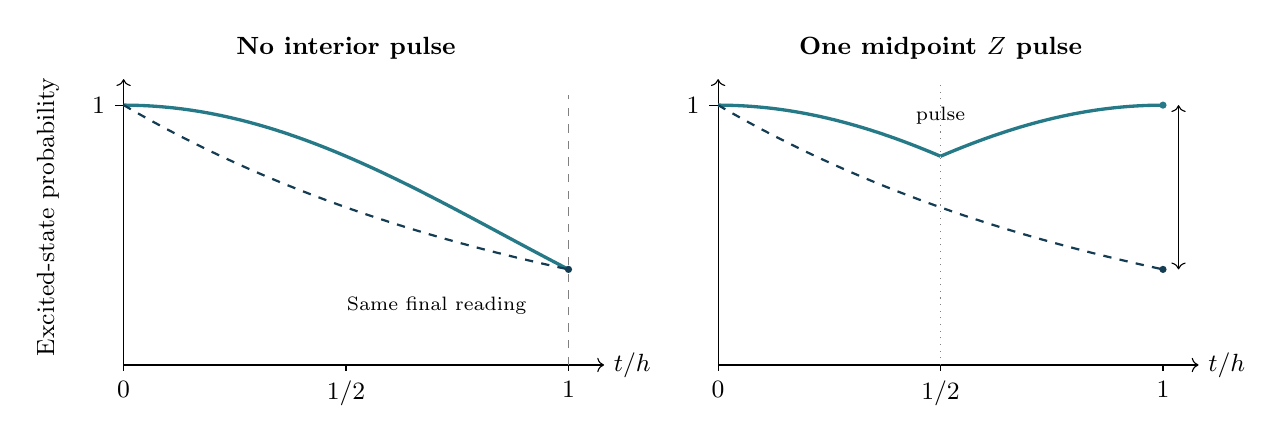
\begin{tikzpicture}[x=5.65cm,y=3.3cm,font=\small]
\begin{scope}
\node[font=\small\bfseries] at (0.5,1.22) {No interior pulse};
\draw[->] (0,0) -- (1.08,0) node[right] {$t/h$};
\draw[->] (0,0) -- (0,1.1);
\node[rotate=90] at (-0.17,0.57) {Excited-state probability};
\foreach \x/\lab in {0/0,0.5/{1/2},1/1}
 {\draw (\x,0) -- (\x,-0.025) node[below] {$\lab$};}
\draw (0,1) -- (-0.02,1) node[left] {$1$};
\draw[dashed,gray] (1,0) -- (1,1.04);
\draw[accent,very thick,domain=0:1,samples=100]
 plot (\x,{cos(acos(exp(-0.5))*\x)^2});
\draw[ink,thick,dashed,domain=0:1,samples=100]
 plot (\x,{exp(-\x)});
\fill[ink] (1,{exp(-1)}) circle[radius=1.3pt];
\node[anchor=west,font=\scriptsize] at (0.48,0.23) {Same final reading};
\end{scope}
\begin{scope}[xshift=7.55cm]
\node[font=\small\bfseries] at (0.5,1.22) {One midpoint $Z$ pulse};
\draw[->] (0,0) -- (1.08,0) node[right] {$t/h$};
\draw[->] (0,0) -- (0,1.1);
\foreach \x/\lab in {0/0,0.5/{1/2},1/1}
 {\draw (\x,0) -- (\x,-0.025) node[below] {$\lab$};}
\draw (0,1) -- (-0.02,1) node[left] {$1$};
\draw[gray,dotted] (0.5,0) -- (0.5,1.08);
\node[font=\scriptsize] at (0.5,0.96) {pulse};
\draw[accent,very thick,domain=0:0.5,samples=60]
 plot (\x,{cos(acos(exp(-0.5))*\x)^2});
\draw[accent,very thick,domain=0.5:1,samples=60]
 plot (\x,{cos(acos(exp(-0.5))*(1-\x))^2});
\draw[ink,thick,dashed,domain=0:1,samples=100]
 plot (\x,{exp(-\x)});
\fill[accent] (1,1) circle[radius=1.3pt];
\fill[ink] (1,{exp(-1)}) circle[radius=1.3pt];
\draw[<->] (1.035,{exp(-1)}) -- (1.035,1);
\end{scope}
\end{tikzpicture}

{\small\textcolor{accent}{Solid: microscopic exchange}\qquad
\textcolor{ink}{Dashed: Markov decay}}
\caption{The same endpoint can conceal different dynamics.
These are exact excited-population curves for the example $\gamma h=1$,
with $\theta=\arccos(e^{-1/2})$. Without the pulse, both final populations
are $e^{-1}$. With the pulse, the microscopic exchange is undone and its
population returns to one; the Markov decay continues. The proof above
establishes equality of the whole endpoint channel in the unpulsed experiment,
not just equality of these plotted populations.}
\label{fig:echo}
\end{figure}

\subsection{An exact cell for a general dissipator}
\label{sim:general-cell}

Return to the centered, drift-free generator and its positive loss operator
$Q=\sum_a M_a^\dagger M_a$, with $\|Q\|=\nu$. The system dimension is
$d$. We seek a finite bath and a time-independent Hamiltonian for one cell
whose reduced endpoint channel is exactly $e^{h\mathcal L}$. The same
Hamiltonian will also have the symmetry needed to bound interrupted cells.

First isolate one particularly useful Kraus operator,
\begin{equation}
 A_0=e^{-hQ/2}.
 \label{sim:nojump}
\end{equation}
It is a positive operator: all its eigenvalues are positive real numbers.
It represents the no-jump contribution. This is an algebraic decomposition
of the channel, not a claim that the tester observes environmental jumps.

To justify it, split the generator into
\begin{equation}
 \mathcal L=\mathcal G+\mathcal J,\qquad
 \mathcal G(\rho)=-\tfrac12\{Q,\rho\},\qquad
 \mathcal J(\rho)=\sum_aM_a\rho M_a^\dagger.
 \label{sim:generator-split}
\end{equation}
The propagation $e^{s\mathcal G}(\rho)=e^{-sQ/2}\rho e^{-sQ/2}$
and the map $\mathcal J$ are completely positive. Expanding the full
propagator according to the number of inserted $\mathcal J$ maps yields
\begin{equation}
 e^{h\mathcal L}=e^{h\mathcal G}
 +\int_0^h e^{(h-t)\mathcal G}\mathcal J e^{t\mathcal G}\,\dd t
 +\text{terms with two or more insertions}.
 \label{sim:positive-expansion}
\end{equation}
Each later term is an ordered integral of completely positive maps. The
series converges in finite dimension. Consequently the remainder after
subtracting $A_0(\cdot)A_0$ is completely positive. Nothing in this
argument assumes that the jumps commute with one another or with $Q$.

Choose Kraus operators $B_1,\ldots,B_s$ for this remainder, with
$s\le d^2$, and regard them as one column operator $B$. In plain terms,
$B$ sends a system vector to the column containing all the vectors $B_a$
would produce. Because the entire channel preserves trace,
\begin{equation}
 A_0^2+B^\dagger B=I.
 \label{sim:column-normalization}
\end{equation}
This is the condition that the total probability in the no-jump and
remaining branches adds to one.

We now convert that column into an actual unitary motion. In a scalar
example, if a real amplitude $0\le a\le1$ remains in the original sector, the amplitude
transferred elsewhere must have length $\sqrt{1-a^2}$. A rotation through
$\arccos a$ has precisely these cosine and sine components. We apply
that construction in each eigenvector direction of $A_0$. Define the angle
operator $\Theta=\arccos A_0$ by diagonalizing $A_0$ and applying
$\arccos$ to each eigenvalue. Its eigenvalues lie in $[0,\pi/2)$.
The polar decomposition of $B$ has the form
\begin{equation}
 B=J\sin\Theta,
 \qquad J^\dagger J=P_\Theta,
 \label{sim:polar}
\end{equation}
where $P_\Theta$ projects onto the support of $\Theta$: the subspace
with nonzero angle. The map $J$ preserves lengths on that subspace and
maps it into the excited bath sectors. It may vanish on the orthogonal
subspace; this is why it is called a partial isometry. If an angle is
zero, there is no amplitude to rotate into the bath. We never divide by
that angle or by its sine, so a rank-deficient loss operator causes no
singularity.

Give the bath a vacuum state $|0\rangle$ and $s$ excited labels
$|1\rangle,\ldots,|s\rangle$. Decompose the joint Hilbert space into
the vacuum sector and the direct sum of the excited sectors. On this
space set
\begin{equation}
 K_h=\frac1h
 \begin{pmatrix}
 0&-i\Theta J^\dagger\\
 iJ\Theta&0
 \end{pmatrix}.
 \label{sim:rotation-generator}
\end{equation}
The off-diagonal blocks are adjoints of one another, so $K_h$ is a
Hermitian Hamiltonian. For each eigenvector with angle $\vartheta>0$,
it generates an ordinary two-dimensional rotation between that vector
in the vacuum sector and its image under $J$. The zero-angle sector
and unused excited directions are left fixed. Therefore
\begin{equation}
 e^{-ihK_h}\begin{pmatrix}I\\0\end{pmatrix}
 =\begin{pmatrix}\cos\Theta\\J\sin\Theta\end{pmatrix}
 =\begin{pmatrix}A_0\\B\end{pmatrix}.
 \label{sim:rotation-column}
\end{equation}
This equation specifies the unitary's action for a vacuum bath and every
system input. Taking the bath trace gives precisely the desired Kraus
channel, and hence precisely $e^{h\mathcal L}$.

Its norm is controlled by the largest rotation angle:
\begin{equation}
 h\|K_h\|=\|\Theta\|
 =\arccos(e^{-\nu h/2})=:\theta_h,
 \qquad \theta_h^2\le\nu h.
 \label{sim:angle-bound}
\end{equation}
For the last inequality, use
$-2\log\cos\theta=2\int_0^\theta\tan u\,\dd u\ge\theta^2$,
because $\tan u\ge u$ for $0\le u<\pi/2$. Here $\log$ is the natural
logarithm. This proves $\|K_h\|\le\sqrt{\nu/h}$.

Finally, let bath parity assign sign $+1$ to its vacuum and sign $-1$
to every excited label:
\begin{equation}
 Z_E=|0\rangle\langle0|-\sum_{a=1}^s|a\rangle\langle a|.
 \label{sim:bath-parity}
\end{equation}
Conjugating $K_h$ by $I_S\otimes Z_E$ changes the signs of both
off-diagonal blocks, so it sends $K_h$ to $-K_h$. The initial bath
state is unchanged. This symmetry is the extra property that will
control arbitrary interruptions; an arbitrary endpoint dilation would
not automatically supply it.

\subsection{From one cell to one admissible finite bath}
\label{sim:grid}

Recall $T=1/\nu$, $\Lambda\ge\nu$ and $q=(\nu/\Lambda)^2$.
Choose the number of collision cells and their duration as
\begin{equation}
 M_{\mathrm c}=\lfloor1/q\rfloor,\qquad
 h=\frac{T}{M_{\mathrm c}},\qquad
 x=\nu h=\frac1{M_{\mathrm c}}.
 \label{sim:grid-choice}
\end{equation}
The floor $\lfloor y\rfloor$ denotes the largest integer no larger
than $y$. Since $1/q\ge1$, we have $M_{\mathrm c}\ge1$ and
$x\le1$. Also $\lfloor y\rfloor\ge y/2$ for $y\ge1$, so $x\le2q$.

Prepare all $M_{\mathrm c}$ bath cells in their vacuum states at time
zero. Couple the system to cell 1 for the first interval, to cell 2 for
the second, and so on. Each cell is retained after use but never coupled
again. ``Fresh'' here means previously unused, not newly supplied or
reset during the experiment. The strength satisfies
\begin{equation}
 \|K_h\|\le\sqrt{\frac\nu h}
 =\nu\sqrt{M_{\mathrm c}}\le\Lambda.
 \label{sim:grid-strength}
\end{equation}
The model is therefore admissible. Crucially, neither $M_{\mathrm c}$
nor the switching schedule depends on the contact budget $N$, the
chosen input, or a measurement outcome. This one device will supply
the upper bound for every $N$.

An untouched cell has exactly the target endpoint action. Previously
used cells may be correlated with the tester, but never interact again;
tracing them out cannot change later tester statistics. Future cells
remain in their initial independent states. These facts allow us to
treat each next cell as a channel on the accessible system, memory
and records. They are properties of this construction, not assumptions
that an arbitrary physical bath can be reset.

\subsection{Why even a complicated interrupted cell has small error}
\label{sim:cell-bound}

Fix any allowed control subroutine during one cell. Keep its input,
protected reference, instruments, classical records and feedback rules
identical in three experiments: the microscopic cell, the target Markov
cell, and an idle cell in which the system does not evolve between
contacts. Denote their complete output channels by $\mathcal F_D$,
$\mathcal F_M$ and $\mathcal F_0$. The idle experiment is a mathematical
comparison; it is not an extra noise-free setting granted to the tester.

Start with a finite adaptive protocol tree. Collect all the contact times
appearing on its branches into one ordered list. At each time apply the
prescribed instrument controlled by the earlier record, using the identity
on branches that have no contact then. Retain every outcome. This represents
the same adaptive experiment as a sequence of trace-preserving channels.
It does not charge the union of those times as the contact budget; it is
only a convenient representation for the following single-cell estimate.

Multiply the microscopic Hamiltonian by a real scalar $\alpha$ and
expand the resulting output channel as a power series,
\begin{equation}
 \mathcal F_{\alpha K_h}
 =\sum_{k=0}^\infty\alpha^k\mathcal F^{(k)},
 \qquad \|\mathcal F^{(k)}\|_\diamond
 \le\frac{(2\theta_h)^k}{k!}.
 \label{sim:dyson-bound}
\end{equation}
Each insertion of the Hamiltonian commutator has diamond norm at most
$2\|K_h\|$. The maps between insertions have norm one. Integrating
over ordered insertion times supplies the factor $h^k/k!$, which proves
the displayed estimate. The bound includes arbitrarily large finite
protected references and all classical outputs.

Bath parity changes $\alpha$ to $-\alpha$. It leaves the initial
vacuum unchanged, commutes with every tester operation, and disappears
when the bath is finally traced out. Hence
$\mathcal F_{\alpha K_h}=\mathcal F_{-\alpha K_h}$. Every odd coefficient
in the power series must vanish. Since its zero-order term is the idle
experiment, summing the remaining terms gives
\begin{equation}
 \frac12\|\mathcal F_D-\mathcal F_0\|_\diamond
 \le\frac12\sum_{k=1}^\infty\frac{(2\theta_h)^{2k}}{(2k)!}
 =\sinh^2\theta_h.
 \label{sim:even-bound}
\end{equation}
Here $\sinh u=(e^u-e^{-u})/2$ and $\cosh u=(e^u+e^{-u})/2$.
The missing linear term matters: $\theta_h$ is of order $\sqrt{x}$,
whereas the desired discrepancy is of order $x$.

For the target-to-idle comparison, replace the Markov evolution by idle
one infinitesimal interval at a time. The unchanged preceding and following
physical maps contract trace distance. Integrating the generator norm
$\|\mathcal L\|_\diamond=2\nu$ over the cell yields
\begin{equation}
 \frac12\|\mathcal F_M-\mathcal F_0\|_\diamond\le\nu h=x.
 \label{sim:markov-idle}
\end{equation}
The triangle inequality now bounds the actual cell discrepancy by
\begin{equation}
 \frac12\|\mathcal F_D-\mathcal F_M\|_\diamond
 \le\sinh^2\theta_h+x
 \le\cosh^2(1)x=:\varepsilon_{\mathrm{cell}}.
 \label{sim:complete-cell-error}
\end{equation}
Indeed $\theta_h\le\sqrt{x}\le1$, and convexity gives
$\sinh u\le u\sinh1$ for $0\le u\le1$. Combining this with
$\cosh^2 1=1+\sinh^2 1$ proves the last inequality.
The estimate is independent of how many contacts the subroutine makes
inside this cell. It concerns the complete output with its failure
branches included, never a normalized rare selected outcome.

\subsection{Adaptive timing still pays only for the cells actually touched}
\label{sim:adaptive}

Call a cell \emph{active} if it contains a system contact strictly inside
its interval. A contact exactly at a cell boundary still uses the tester's
budget, but lies between two matched endpoint channels. It need not be
charged as an active cell. On any realized history, at most $N$ cells
are active. The difficulty is that different histories can activate
different cells. Their union might contain far more than $N$ cells.

For example, suppose a fair coin chooses whether the sole contact occurs
in cell 1 or cell 2. Two cells appear in the list of all possibilities,
but each actual run uses one contact. Their activation probabilities are
$p_1=p_2=1/2$, and $p_1+p_2=1$. The proof must preserve this accounting
even when the choice is made by a measurement on an entangled memory.

We first put the decision to activate a cell at a well-defined place.
Before its first system contact, the tester can only act on its protected
memory $R$. A branch map $\mathcal A_R$ commutes with any joint
system--bath propagation $\mathcal U_{SE}$:
\begin{equation}
 (\mathcal U_{SE}\otimes\mathrm{id}_R)
 (\mathrm{id}_{SE}\otimes\mathcal A_R)
 = (\mathrm{id}_{SE}\otimes\mathcal A_R)
 (\mathcal U_{SE}\otimes\mathrm{id}_R).
 \label{sim:memory-commutation}
\end{equation}
This operator identity holds on entangled inputs too. A memory measurement
may change the conditional system--bath state, but moving the same branch
map through the propagation preserves that subnormalized state and its
probability. Commutation is not an independence assumption.

Collect the memory-only operations up to the first system contact or the
cell's end, whichever comes first. Move those operations to the entrance
using \eqref{sim:memory-commutation}, retaining their outcomes and the
originally selected first-contact time. The resulting entrance instrument
declares either an active cell and its first-contact time, or no contact
inside the cell. Nothing from after the cell is moved backward. Later
contacts in an active cell remain fully adaptive. This is a representation
of the same controller, not an extra information channel or a free move
of a physical system contact.

Let $\Phi_j$ and $\Psi_j$ be the complete microscopic and target channels
for cell $j$, including that common entrance instrument and the tester's
subroutine. For an input state $\rho$, let $p_j(\rho)$ be its active-flag
probability. The inactive outputs agree exactly. The active outputs obey
\eqref{sim:complete-cell-error}; multiplying their normalized bound by
the probability of that branch gives
\begin{equation}
 \frac12\|(\Phi_j-\Psi_j)(\rho)\|_1
 \le\varepsilon_{\mathrm{cell}}p_j(\rho).
 \label{sim:weighted-cell}
\end{equation}
Complete records keep different entrance outcomes in separate classical
blocks, so these weighted estimates add without discarding information.

To compare the whole experiment, replace its cells one at a time using
the telescoping identity
\begin{equation}
 \Phi_{M_{\mathrm c}}\cdots\Phi_1-
 \Psi_{M_{\mathrm c}}\cdots\Psi_1
 =\sum_{j=1}^{M_{\mathrm c}}
 \Psi_{M_{\mathrm c}}\cdots\Psi_{j+1}
 (\Phi_j-\Psi_j)\Phi_{j-1}\cdots\Phi_1.
 \label{sim:hybrid}
\end{equation}
In each summand the preceding part is the genuine microscopic execution,
and the following part is a target channel that contracts the discrepancy.
Thus every activity weight comes from one and the same probability law,
the full microscopic experiment. Writing $p_j$ for those probabilities,
\begin{align}
 \frac12\|\rho_D^{\mathsf T}-\rho_M^{\mathsf T}\|_1
 &\le\varepsilon_{\mathrm{cell}}\sum_{j=1}^{M_{\mathrm c}}p_j,
 \nonumber\\
 \sum_{j=1}^{M_{\mathrm c}}p_j
 &=\E_D[\text{number of active cells}]\le N.
 \label{sim:actual-budget}
\end{align}
The expectation is bounded because every history obeys the hard contact
budget. A rare branch does not receive free contacts, and mutually
exclusive branches are not counted as though they occurred together.

Finally, $x=1/M_{\mathrm c}\le2q$ and a final binary readout cannot
increase trace distance. The constructed device therefore obeys, for
every allowed tester,
\begin{equation}
 |p_D^{\mathsf T}-p_M^{\mathsf T}|
 \le\min\{1,2\cosh^2(1)Nq\}.
 \label{sim:global-upper}
\end{equation}
The argument directly covers finite protocol trees at arbitrary real
contact times. The bound survives the stipulated operational limits of
such controllers, since it is uniform and their output probabilities
converge. This does not enlarge the model to coherent superpositions of
contact times or uncounted continuous monitoring.

\subsection{What the two directions establish}
\label{sim:consequences}

Combining this single-device upper bound with the universal survival
witness gives
\begin{equation}
 \frac1{64}\min\{1,Nq\}\le\Gamma_N\le\Delta_N
 \le\min\{1,2\cosh^2(1)Nq\},
 \qquad q=\frac{\nu^2}{\Lambda^2}.
 \label{sim:matched-law}
\end{equation}
The lower tester does not know the microscopic bath. The upper simulator
does not know which tester will be used. These complementary uniform
statements establish a contact cost of order $(\Lambda/\nu)^2$ for
a fixed positive single-run distinguishing advantage. They do not assert
an exact threshold or optimal numerical constants.

At $N=0$, every cell is inactive, so their exact endpoint channels compose
to $e^{T\mathcal L}$. This particular microscopic model is indistinguishable
from the target by every terminal measurement, including reference-assisted
ones. Hence $\Gamma_0=\Delta_0=0$. This is an existence statement about
a hiding model; other microscopic models may already have a different
endpoint. An earlier system readout is a paid interior contact, even if
its result is stored until $T$.

The same theorem can be read as a strength requirement for simulation.
Let $\Lambda_{\min}(N,\epsilon)$ be the infimum of allowed strengths
for which some microscopic model keeps the worst permitted tester's
probability gap at most $\epsilon$. For $N\ge1$ and
$0<\epsilon<1/64$, the lower bound forces its unsaturated branch;
otherwise its gap would already be at least $1/64$. Inverting the two
inequalities gives
\begin{equation}
 \nu\sqrt{\frac{N}{64\epsilon}}
 \le\Lambda_{\min}(N,\epsilon)
 \le\nu\sqrt{\frac{2\cosh^2(1)N}{\epsilon}}.
 \label{sim:strength-cost}
\end{equation}
In words, tolerating more interventions or demanding smaller error
requires a larger microscopic strength, proportional to
$\nu\sqrt{N/\epsilon}$ in this model.

There are costs outside that statement. Each general cell has at most
$d^2+1$ bath levels, so the complete bath used here has dimension at most
$(d^2+1)^{M_{\mathrm c}}$. For the explicit qubit exchange construction it
is $2^{M_{\mathrm c}}$. All those cells are prepared at time zero; the
schedule is externally prescribed. The result neither bounds the effort
of preparing that bath nor supplies an autonomous clock or finite-duration
instruments. Independent repetitions of the whole duration-$T$ experiment
are also additional resources. The theorem is a precise statement about
interaction strength and counted contacts, with these other resources
stated openly.

We have now completed the discrimination argument. The next question asks
what temporal access can \emph{enable} in an estimation task. A visible
difference between two processes does not itself provide a precise
frequency estimate. That requires a separate device, estimator and
lower-bound argument.


\section{What a record comparison does, and does not, tell us about sensing}
\label{bridge:section}

The resolution theorem compares two descriptions of a controlled experiment.
An estimation theorem asks how accurately a number can be inferred from its
data. These questions are related, but neither answers the other by itself.
A measurement can reveal that a noise model is inaccurate without revealing
much about the frequency we want. Conversely, microscopic memory can make
the actual sensor more useful than the memoryless model predicts.

This section makes the connection precise for one simple device. It also
explains why the global sensing theorem that follows needs an explicit
estimator, a fixed frequency band and a separate lower bound.

\subsection{A parity record can test the noise model}

Take a sensor qubit $S$ and a protected ancilla qubit $A$; an ancilla
is an additional quantum system used to prepare or read the experiment.
Use the Pauli matrices defined in \eqref{eq:pauli}.
The operator $Z_SZ_A$ means $Z_S\otimes Z_A$. Its even sector is spanned
by $|00\rangle,|11\rangle$, and its odd sector by $|10\rangle,|01\rangle$.
Measuring its sign is a parity measurement. It tells us whether a transverse
sensor flip occurred an odd number of times, without distinguishing the
two basis states inside the same sector. The even projector is
$\Pi=(I+Z_SZ_A)/2$.

A transverse error has the form
\begin{equation}
 N_\phi=\cos\phi\,X_S+\sin\phi\,Y_S,
 \qquad N_\phi^2=I,
 \qquad N_\phi Z_S N_\phi=-Z_S.
\end{equation}
The angle $\phi$ is unknown but fixed across the experiment. Two identical
flips cancel, while a flip reverses the sign of subsequent signal phase.
Let $\epsilon=\omega-\omega_0$ be the unknown frequency relative to a fixed
nominal compensation $\omega_0$. The compensation is a physical setting;
calculating a new classical estimate does not change it.

For this bridge, a Markov device accepts a classical rate command
$\gamma\in\{a,b\}$, with fixed known $0<a<b$, and has generator
\begin{equation}
 \mathcal L_{\epsilon,\phi,\gamma}(\rho)
 =-i\frac\epsilon2[Z_S,\rho]
 +\gamma(N_\phi\rho N_\phi-\rho).
 \label{bridge:markov-model}
\end{equation}
The rate command is an explicit input port of this model. It is not an
extra free control secretly inserted into the preceding fixed-generator
theorem. The sensing theorem in the next section will instead hold one
microscopic coupling fixed.

Start even, check parity every $\Delta$ units of time, and use rate $a$
after an even result and $b$ after an odd result. Let $E_n$ be the event that
all $n$ checks are even, with $T=n\Delta$. This event includes hidden pairs
of errors between checks; it is not a no-error event. Under the Markov law,
every interval along the all-even history uses rate $a$. With that
setting, the instantaneous jump rate is $a$, independent of the sensor state,
because $N_\phi^\dagger N_\phi=I$. The number $K$ of jumps in one
interval has the Poisson probabilities
\begin{equation}
 \Pr(K=k)=e^{-a\Delta}\frac{(a\Delta)^k}{k!},
 \qquad k=0,1,2,\ldots .
\end{equation}
Here $k!=1\cdot2\cdots k$, with $0!=1$, and the mean count is $a\Delta$.
Summing the even terms gives
\begin{equation}
 \Pr_M(E_n)=\left(\frac{1+e^{-2a\Delta}}2\right)^n.
 \label{bridge:even-record}
\end{equation}
For example, the identity follows by adding the exponential series for
$e^{a\Delta}$ and $e^{-a\Delta}$ and dividing by two, then multiplying
by $e^{-a\Delta}$. The signal preserves parity and cannot change this
probability.

Now suppose a competing microscopic device has a parity-preserving
Hamiltonian part and a parity-changing part bounded by $\Lambda_\perp$.
Bath-only motion and the signal can be included in the preserving part.
The same subspace-survival argument as before gives
\begin{equation}
 \Pr_D(E_n)\ge\cos^{2n}(\Lambda_\perp\Delta),
 \qquad 0\le\Lambda_\perp\Delta\le\pi/2.
\end{equation}
It remains valid after each success despite the conditional bath state.
Consequently the total variation of the \emph{complete} record distributions
is at least
\begin{equation}
 \max\left\{0,\cos^{2n}(\Lambda_\perp\Delta)
 -\left(\frac{1+e^{-2a\Delta}}2\right)^n\right\}.
\end{equation}
At fixed $T$ and fixed $\Lambda_\perp$, taking $\Delta=T/n\to0$ makes this
certificate tend to $1-e^{-aT}$. At fixed positive $\Delta$ and growing
$T$, both all-even probabilities may instead tend to zero. The order of
limits therefore matters. Also, a bound on parity-changing noise is not
the complete system-affecting bound $\Lambda$ of
\eqref{eq:complete-strength}; it need not constrain a large diagonal signal.

\subsection{One microscopic device approximating complete records}

For a specified cell duration $h$, choose the coupling associated with a
rate command as
\begin{equation}
 p_\gamma=\frac{1-e^{-2\gamma h}}2,
 \qquad \theta_\gamma=\arcsin\sqrt{p_\gamma},
 \qquad g_\gamma=\frac{\theta_\gamma}{h}.
\end{equation}
Each cell couples the sensor to one bath qubit initially in $|0\rangle$,
using
\begin{equation}
 H_\gamma=\frac\epsilon2 Z_S\otimes I_E+
 g_\gamma N_\phi\otimes X_E.
\end{equation}
All bath qubits are supplied at time zero and retained after use. At
$\epsilon=0$, tracing the bath gives exactly the Markov cell channel in
\eqref{bridge:markov-model}: its flip probability is $p_\gamma$.
For $|\epsilon|\le W$, the complete interaction norm is at most
$\sqrt{g_b^2+W^2/4}$. Reporting $g_b$ alone as that norm would omit the signal.

With the signal present, the exact collision channel $\mathcal C_\gamma$
and the Markov channel obey the uniform one-cell estimate
\begin{equation}
 \frac12\|\mathcal C_\gamma-e^{h\mathcal L_{\epsilon,\phi,\gamma}}
 \|_\diamond
 \le\frac{|\epsilon|h}{2}
 [\theta_\gamma\sinh(2\theta_\gamma)+\gamma h]
 \le 2|\epsilon|\gamma h^2.
 \label{bridge:cell-error}
\end{equation}
Here $\sinh x=(e^x-e^{-x})/2$. To see the important small-time order,
remove the signal by its interaction picture. The rotating error operator
satisfies $\|N_\phi(t)-N_\phi(0)\|\le|\epsilon|t$. Odd bath terms vanish
by the same parity symmetry used for the controlled-cell theorem. At even
order $k$ of the time-ordered expansion, telescoping the $k$ coupling
factors and integrating their
time arguments bounds the half-diamond difference by terms whose sum is
\begin{equation}
 \frac{|\epsilon|h}{4}
 \sum_{\substack{k\ge2\\k\ \mathrm{even}}}
 \frac{k(2\theta_\gamma)^k}{k!}
 =\frac{|\epsilon|h\theta_\gamma}{2}\sinh(2\theta_\gamma).
\end{equation}
The rotating Markov dissipator contributes at most
$\gamma|\epsilon|h^2/2$ by the contractive integral comparison.
Finally, $\theta_\gamma<\pi/4$ and
$\theta_\gamma^2\le\gamma h$ give the last bound in
\eqref{bridge:cell-error}. The cancellation of odd terms is what avoids
a weaker square-root-in-time estimate.

Restrict commands and system instruments to cell boundaries. Keeping all
records and replacing cells one at a time then gives, over $T/h$ cells,
\begin{equation}
 \mathrm{TV}(P_D,P_M)\le\delta(T,h),
 \qquad \delta(T,h)=\min\{1,2WbTh\}.
 \label{bridge:record-error}
\end{equation}
Each complete adaptive boundary instrument is a channel and contracts the
error. The uniform cell bound applies to every conditional input and
selected rate, so no number-of-branches factor appears. Readouts finishing
early can be stored through the remaining charged horizon. Inside-cell
operations are outside this particular comparison.

A \emph{loss} is a numerical penalty assigned to an estimate; its average
is the \emph{risk}. Squared frequency error is the loss used below.
If a loss takes values between zero and $B$, its expectation changes by
at most $B\,\delta(T,h)$ between these two record laws. For a frequency
interval of width $L$, clipping the estimate to the interval makes squared
loss at most $L^2$. Thus the \emph{same} estimator and experiment have
risks differing by at most $L^2\delta(T,h)$. The same conclusion survives
optimization if both models use the same strategy class and parameter domain.
Clipping means replacing an answer outside the interval by its nearest
endpoint. This cannot move the answer farther from a true frequency
inside the interval.

This is a finite-horizon error-transfer bound. Two models can predict
almost the same records while their remaining difference is still larger
than the tiny estimation error we seek. The comparison therefore cannot
replace a direct precision proof. It also does not say that a
small total-variation error controls frequency derivatives. For instance,
a small function can vary rapidly as its argument changes. Local Fisher
information depends on derivatives of probabilities and therefore needs
another argument. Likewise, taking $h$ smaller improves
\eqref{bridge:record-error} but increases the required coupling,
$g_\gamma\sim\sqrt{\gamma/h}$, as well as the number of preinitialized bath
cells. A fixed-strength global sensing result cannot be obtained by making
these resources grow without charging them. We now hold the hardware fixed
and solve the estimation task directly.

\subsection{Why an identifiable frequency band is a real condition}

Watching a clock hand only at fixed intervals can hide whole extra turns.
Different rotation speeds can then produce exactly the same readings.
In estimation this is called an \emph{alias}. An identifiable band is a
promised frequency interval on which the available observations can
distinguish different frequencies. More data cannot resolve an exact alias
if every new observation repeats the same ambiguity.

Fix one coupling $g>0$ and cell duration $h$, let $\chi=gh<\pi/4$, and
retain the simultaneous Hamiltonian
$H=(\epsilon/2)Z_S\otimes I+gN_\phi\otimes X_E$.
Its two terms anticommute, so
$H^2=R(\epsilon)^2I$ with
$R(\epsilon)=\sqrt{g^2+\epsilon^2/4}$. Its exact propagator is
\begin{equation}
 e^{-ihH}=\cos(Rh)I-i\frac{\sin(Rh)}R H.
\end{equation}
For any positive integer $k$, both residual frequencies
\begin{equation}
 \epsilon_k^\pm=\pm\frac2h\sqrt{k^2\pi^2-\chi^2}
\end{equation}
give $Rh=k\pi$ and hence $e^{-ihH}=(-1)^k I$. The scalar sign cannot be
observed. Every complete cell is the identity channel, independently of
the nuisance direction.

Any controller restricted to cell boundaries consequently obtains the
same complete data at two such resonant frequencies. This remains true
with adaptation: equal input states and records lead through the same
identity cell to equal boundary-instrument outcome laws; induction repeats
the statement through every cell. Let the two frequencies be $\omega_1$
and $\omega_2$, separated by $D=|\omega_1-\omega_2|$. Their common estimate
distribution obeys
\begin{equation}
 \frac12\sum_{j=1}^2\E_{\omega_j}
       [(\widehat\omega-\omega_j)^2]
 =\E[(\widehat\omega-(\omega_1+\omega_2)/2)^2]+\frac{D^2}{4}
 \ge\frac{D^2}{4}.
\end{equation}
At least one frequency must have that much squared error, however many
cells are used. This is an exact ambiguity, not merely a noisy estimate.
Only resonances lying in the permitted frequency domain matter; its full
Hamiltonian bound must also allow their strength $k\pi/h$.

The theorem below uses a fixed nonzero band near compensation where a
simple calibration measurement is uniformly informative. The band does
not shrink as the experiment grows. It is a sufficient identifiable band,
not a claim of maximum bandwidth. The alias argument concerns boundary
access at one fixed coupling and clock; it is not an obstruction proved
for every possible inside-cell control.


\section{How many resolved collisions improve an unknown frequency?}
\label{con:task}

We now ask for an estimate rather than a yes-or-no decision. The frequency
is initially unknown on a fixed interval. The aim is to make its largest
mean-square estimation error small, even when the direction of the noise
is also unknown. The discrimination theorem does not answer this question:
a detectable difference between two devices need not provide a useful,
unambiguous frequency reading. We need both an actual estimator and a bound
that applies to every permitted estimator.

\subsection{The fixed device and the two contact budgets}

The sensor is a qubit $S$, with a protected ancillary qubit available for
the constructions and arbitrary finite protected memory allowed in the
comparison. Its frequency is $\omega$. A fixed known compensation frequency
$\omega_0$ leaves the residual frequency $\epsilon=\omega-\omega_0$.
Each interaction cell lasts $h>0$. During a cell the sensor and its assigned
bath qubit evolve under
\begin{equation}
 H(\epsilon,\phi)=\frac{\epsilon}{2}Z_S\otimes I_E
       +gN_\phi\otimes X_E,
 \qquad N_\phi=\cos\phi\,X_S+\sin\phi\,Y_S.
 \label{con:H}
\end{equation}
The coupling $g>0$ is fixed, and $\chi=gh$ lies in $(0,\pi/4)$.
The same unknown direction $\phi$ applies throughout all cells and repeated
trials. All bath qubits begin in $|0\rangle$ at time zero; after use they
remain inaccessible and never interact again. Thus the construction uses
new partners already present in the finite bath, not uncharged resets of
an exposed environmental qubit.

There are $n$ cells and a hard duration $T=nh$. At most $n-1$ contacts may
act on the sensor strictly before the final time; at most $m$ of them may
occur strictly inside cells, where $0\le m\le n-1$. Both restrictions hold
on every classical history. Preparations at time zero and readout at $T$
are free. A readout earlier than $T$ counts, even if its result is stored
until $T$. Boundary operations performed at the same instant may be combined
into one instrument. Neither feedback nor a frequency estimate changes the
physical compensation, the coupling or the collision clock.

The counts have different jobs. In the resolution theorem, $N$ counted
all intermediate contacts in a fixed-time comparison over many devices.
Here $n$ counts the interaction cells of this particular sensor, and $m$
counts contacts strictly inside them. Cell boundaries are not interior
access, but operations there still consume the total contact allowance.

The comparison allows finite adaptive instrument trees, their
parameter-independent classical mixtures, and limits whose event
probabilities converge on an open parameter neighborhood while keeping
the same structural budgets. Classical feedback may select real contact
times. It does not grant coherent superpositions of times or continuous
uncounted monitoring between contacts.

Choose a fixed interval $\Omega=[\omega_0-E,\omega_0+E]$, with $E>0$ to be
specified. Its width does not shrink as $n$ grows. For an allowed procedure
$\mathcal P$ and its numerical answer $\widehat\omega$, the risk is
$\mathbb E_{\omega,\phi}^{\mathcal P}(\widehat\omega-\omega)^2$.
The expectation averages every outcome, including unsuccessful records.
The optimal worst-case risk is
\begin{equation}
 R_{n,m}^*(\Omega)=\inf_{\mathcal P,\widehat\omega}
 \sup_{\omega\in\Omega,\phi}
 \mathbb E_{\omega,\phi}^{\mathcal P}
       (\widehat\omega-\omega)^2.
 \label{con:risk}
\end{equation}
The supremum asks for the most difficult allowed frequency and direction;
the infimum selects the best complete experimental procedure. Biased
estimates are allowed. Squared frequency error has units of inverse time
squared.

\begin{theorem}[Global precision with a contact allowance]
For every fixed $g,h$ with $0<gh<\pi/4$, there is a fixed $E>0$ such that
\begin{equation}
 \boxed{R_{n,m}^*(\Omega)
 =\Theta_{\chi,Eh}\!\left(\frac{1}{h^2(n+m^2)}\right)}
 \qquad(n\ge1,\ 0\le m\le n-1).
 \label{con:law}
\end{equation}
The multiplicative constants depend only on the fixed dimensionless
hardware and band parameters $\chi,Eh$, and are uniform in $n,m,\phi$.
\end{theorem}
Here $\Theta$ means upper and lower bounds by positive constant multiples
of the displayed expression. The theorem identifies an order of precision,
not an optimal coefficient or a largest possible frequency band.
When $m=0$, the error has order $1/(h^2n)$. An allowance of order
$\sqrt n$ is the crossover scale. When $m$ is proportional to $n$, the
error has order $1/(h^2n^2)$. We next build the upper bound, then explain
why no permitted adaptive strategy improves its order. Ordinary repeated
readings supply inverse-linear risk in $n$. Interior contacts let useful
phase accumulate over a number of cells proportional to $m$, supplying
inverse-square risk in $m$. We choose the better complete design.
The expression $n+m^2$ does not assume that information from the two
designs can simply be added.

\subsection{One coupling supplies two temporal settings}
\label{con:settings}

Set $R=\sqrt{g^2+\epsilon^2/4}$ and $r=Rh$. Here $R$ is a scalar
frequency scale; the protected quantum memory is a separate system.
The two terms in
\eqref{con:H} anticommute, so $H^2=R^2I$. Consequently its exact propagator
is $\cos r\,I-i(\sin r/R)H$. Reading the two bath components gives the
untouched, or plain, cell operators
\begin{equation}
 K_{0,p}=\cos r\,I-i\frac{\epsilon}{2R}\sin r\,Z_S,
 \qquad K_{1,p}=-i\frac gR\sin r\,N_\phi.
 \label{con:plain}
\end{equation}
The subscript 0 denotes no parity flip, and 1 denotes a flip. Although the
bath is not measured, sensor--ancilla parity distinguishes these branches.
For each branch operator $K$, its probability operator $K^\dagger K$
is a scalar multiple of the identity. Thus each branch probability
is independent of the incoming logical state.

For an echoed cell, insert one sensor $Z_S$ pulse at its midpoint.
The pulse reverses the coupling term and preserves the signal term.
Thus it can undo noise while leaving a signal to measure. With both
terms present, the off-compensation dynamics must still be calculated;
the signal-free echo example alone does not settle it.
A known final $Z_S$ frame correction, performed at the endpoint, changes
its propagator to
\begin{equation}
 V= e^{-iH_-h/2}e^{-iH_+h/2},
 \qquad H_\pm=\frac\epsilon2Z_S\otimes I_E
                   \pm gN_\phi\otimes X_E.
\end{equation}
The frame correction is a real, known $Z_S$ operation that cancels
the extra $Z_S$ left by the interior pulse. It is included in the
endpoint instrument, rather than treated as a free change to the device.
Multiplication of the two half-cell propagators yields
\begin{align}
 V&=(uI-ivZ_S)\otimes I_E-i xN'_\phi\otimes X_E,\nonumber\\
 u&=\cos r+\frac{g^2}{R^2}(1-\cos r),\qquad
 v=\frac\epsilon{2R}\sin r,\qquad
 x=\frac{\epsilon g}{2R^2}(1-\cos r),
 \label{con:echo}
\end{align}
where $N'_\phi=\partial_\phi N_\phi$ and $u^2+v^2+x^2=1$.
An odd outcome of this cell initially applies $N'_\phi$ rather than
$N_\phi$. Apply an additional known $Z_S$ conditional on that outcome.
Because $Z_SN'_\phi=-iN_\phi$, its corrected flip operator is
$-xN_\phi$. The frame correction, parity measurement and conditional
correction are parts of the same endpoint instrument. Only the midpoint
pulse is an inside-cell contact.

Both settings now have the same unknown flip, up to a scalar, and a known
rotation on the no-flip branch. Write
\begin{align}
 p_e&=x^2,&p_p&=\frac{g^2}{R^2}\sin^2r,&q_j&=1-p_j,\nonumber\\
 \theta_e(\epsilon)&=2\arctan(v/u),&&
 \theta_p(\epsilon)=2\arctan\!\left(\frac\epsilon{2R}\tan r\right),
 \label{con:phases}
\end{align}
so $K_{0,j}=\sqrt{q_j}\,e^{-i\theta_jZ_S/2}$ for $j=e,p$.
We restrict the band so $r<\pi/4$; then $u$ and $\cos r$ are positive and
these are smooth, single-valued real phase functions. At compensation,
\begin{equation}
 p_e(0)=0,\qquad p_p(0)=\sin^2\chi,\qquad
 A:=\theta'_e(0)=\frac{\sin\chi}{g},\qquad
 d_p:=\theta'_p(0)=\frac{\tan\chi}{g}.
 \label{con:derivatives}
\end{equation}
Primes on scalar functions mean differentiation with respect to residual
frequency; $A$ and $d_p$ therefore have units of time.
The prime on $N'_\phi$ instead denotes an angle derivative.
The zero echo-flip probability
at $\epsilon=0$ does not make an echoed cell noiseless at every frequency:
$x$ is generally nonzero away from compensation.

\subsection{The recorded path cancels the unknown direction}

Encode a logical qubit using $|0_L\rangle=|00\rangle$ and
$|1_L\rangle=|11\rangle$, and start a block in
$|+_L\rangle=(|0_L\rangle+|1_L\rangle)/\sqrt2$.
A parity measurement reports whether the two physical bits agree, without
asking which of the two code states is present. Denote even parity by
$\sigma=+1$ and odd parity by $\sigma=-1$. Use an echoed cell after an
even result and a plain cell after an odd result. Keep every result.
The odd-state correction above aligns the two flip operators; it does
not return an odd state to even parity.

For a block of $L$ cells, the record is
$\mathcal R=(\sigma_0,\ldots,\sigma_L)$ with $\sigma_0=+1$.
If it ends even, its normalized logical output is exactly
\begin{align}
 |\psi_{\mathcal R}(\epsilon)\rangle
 &=e^{-i\Phi_{\mathcal R}(\epsilon)Z_L/2}|+_L\rangle,\nonumber\\
 \Phi_{\mathcal R}(\epsilon)
 &=\sum_{i=1}^L\sigma_{i-1}
    \mathbf1_{\{\sigma_i=\sigma_{i-1}\}}
    \theta_{j(\sigma_{i-1})}(\epsilon),
 \qquad j(+1)=e,\quad j(-1)=p.
 \label{con:recordphase}
\end{align}
Here $Z_L$ acts as $+1$ on $|0_L\rangle$ and $-1$ on $|1_L\rangle$;
the indicator is one only if that cell did not flip parity.
The logical operators $X_L,Y_L,Z_L$ are the Pauli matrices
\eqref{eq:pauli} in the ordered basis $|0_L\rangle,|1_L\rangle$.
For example, $X_L$ exchanges those two code states and
$Y_L|0_L\rangle=i|1_L\rangle$.
The same calculation as for the qubit clock \eqref{eq:qubit-clock}
gives $\langle X_L\rangle=\cos\Phi_{\mathcal R}$ and
$\langle Y_L\rangle=\sin\Phi_{\mathcal R}$. These are the two
logical readout axes used below.
The explanation is algebraic: $N_\phi^2=I$, while
$N_\phi Z_SN_\phi=-Z_S$. Moving a no-flip rotation past a preceding
flip reverses its phase sign. An even number of the remaining flip factors
then cancels completely. Scalar branch amplitudes determine the record's
probability but do not alter its normalized logical state.

Thus a record gives a known \emph{function} of the candidate frequency,
not an observed value of the unknown frequency. For example, a record
that stays even for three cells has $\Phi=3\theta_e$. A record that
flips into the odd sector, remains there for one plain cell, and then
flips back contributes $-\theta_p$ from that intervening no-flip cell.
The functions and their signs are calculable without knowing $\phi$.
Their probabilities still depend on $\epsilon$; the estimator below keeps
that dependence rather than replacing it by its value at zero.

For a complete four-cell example, follow this recorded path:
\begin{center}
\begin{tabular}{@{}clllc@{}}
\toprule
Cell & Starting parity & Setting & Result & Phase added\\
\midrule
1 & Even & Echo & Stay & $+\theta_e$\\
2 & Even & Echo & Flip & $0$\\
3 & Odd & Plain & Stay & $-\theta_p$\\
4 & Odd & Plain & Flip & $0$\\
\bottomrule
\end{tabular}
\end{center}
Write $U_j=e^{-i\theta_jZ_S/2}$ for a no-flip rotation. Omitting scalar
branch amplitudes, the total operation is
$N_\phi U_pN_\phi U_e=U_p^{-1}U_e$. The unknown direction has
cancelled, and the phase is $\theta_e-\theta_p$. Its slope at zero is
$A-d_p<0$, so this even-ending record will fail the positive-slope
test below. Four even stays instead give phase $4\theta_e$ and slope
$4A$. The flipping path is possible away from compensation; at exact
compensation its echo flip has zero probability.

\subsection{Select records with useful sensitivity over a whole band}
\label{con:gate}

A useful record must have a phase that changes steadily with frequency,
with slope proportional to the block length. The argument below shows
that the mean accumulated slope grows like $L$, while its usual
fluctuations grow only like $\sqrt L$. A threshold below the mean
therefore retains a fixed positive fraction of long blocks.
The frequency band is chosen so that a record passing this test at the
nominal frequency remains sensitive at every candidate frequency.

An even record alone need not have a large net phase derivative: positive
and negative contributions could cancel. We therefore use an observable
record criterion. Choose $E>0$ small enough that, throughout $|\epsilon|\le E$,
\begin{gather}
 r\le r_*:=\sqrt{\chi^2+(Eh/2)^2}<\pi/4,\qquad
 0\le p_e<p_p<\tfrac12,\nonumber\\
 \mu^0(\epsilon):=
 \frac{p_pq_eA-p_e q_p d_p}{p_e+p_p}\ge\frac{3A}{4},\qquad
 \max\{|\theta'_e-A|,|\theta'_p-d_p|\}\le\frac A4.
 \label{con:band}
\end{gather}
These conditions hold on a positive-width interval: at zero,
$p_p>0$, $p_e=0$ and $\mu^0=A$, while the phase derivatives are continuous.
Fix such an interval once. Any separate bound on the complete interaction
must cover $R\le r_*/h$ on it.

Replace each phase derivative in \eqref{con:recordphase} by its value
at zero, obtaining the known number
\begin{equation}
 D_L^0=\sum_{i=1}^L\sigma_{i-1}
 \mathbf1_{\{\sigma_i=\sigma_{i-1}\}}d_{j(\sigma_{i-1})},
 \qquad d_e=A,\quad d_p=\frac{\tan\chi}{g}.
\end{equation}
Accept a record precisely when $\sigma_L=+1$ and $D_L^0\ge AL/2$.
This rule uses measured signs and fixed calibration constants. It does not
assume the true residual frequency is zero.

Here is why a fixed positive fraction of blocks pass. The parity chain has
transition matrix
\begin{equation}
 P=\begin{pmatrix}q_e&p_e\\p_p&q_p\end{pmatrix},\qquad
 \pi_+=\frac{p_p}{p_e+p_p},\qquad
 \lambda=1-p_e-p_p\le\rho<1.
\end{equation}
The final inequality holds uniformly by compactness and $p_p>0$.
Rows and columns of $P$ are ordered even, odd. Its entry in a given row
and column is the probability of moving between those two parities.
The number $\pi_+$ is the long-run even fraction, and $\lambda$ controls
the decay of the initial parity imbalance.
The exact recursion starting even gives
$\Pr(\sigma_i=+1)=\pi_++(1-\pi_+)\lambda^i\ge1/2$.
The stationary average derivative reward is $\mu^0$; starting even adds
a nonnegative transient contribution. Hence
$\mathbb E D_L^0\ge3AL/4$.

For classical random variables, variance and covariance mean
\begin{equation}
 \Var(X)=\E[(X-\E X)^2],\qquad
 \Cov(X,Y)=\E[(X-\E X)(Y-\E Y)].
\end{equation}
Variance measures the spread of an outcome around its mean; covariance
measures whether two fluctuations tend to have the same sign.
The variance tail inequality is
$\Pr(|X-\E X|\ge t)\le\Var(X)/t^2$ for $t>0$:
on that event the squared fluctuation is at least $t^2$.

Let $X_i$ be the $i$th summand of $D_L^0$.
Rewards in nearby cells are correlated, but their correlations decay.
Put $M=\max\{A,d_p\}$ and $V_0=M^2[1+2/(1-\rho)]$.
For rewards $X_i,X_j$ with $i<j$, conditioning on the parity after cell
$i$ leaves a difference between the two possible future mean rewards of
at most $2M\rho^{j-i-1}$. A variable of range length $2M$ has variance
at most $M^2$. Cauchy--Schwarz therefore gives
$|\Cov(X_i,X_j)|\le M^2\rho^{j-i-1}$, and summing the geometric series gives
$\Var(D_L^0)\le V_0L$. The elementary variance tail bound now implies
\begin{equation}
 \Pr(\text{accepted})\ge\frac12-\frac{16V_0}{A^2L}
 \ge\frac14=:p_0
 \quad\text{if }L\ge L_0:=\max\{1,\lceil64V_0/A^2\rceil\}.
 \label{con:acceptance}
\end{equation}
We subtracted the probability of failing the derivative test from the
probability of ending even; these two events need not be independent.
This proof also covers $p_e=0$: an initially even chain is then absorbing,
not an irreducible chain requiring a positive echo-flip probability.

For each accepted record, \eqref{con:band} bounds the change in its
summed derivative by $AL/4$. Thus, at \emph{every candidate frequency}
$v\in[-E,E]$,
\begin{equation}
 \alpha L\le\Phi'_{\mathcal R}(v)\le\beta L,
 \qquad \alpha=A/4,\qquad
 \beta=\max_{j=e,p}\sup_{|v|\le E}|\theta'_j(v)|.
 \label{con:sensitivity}
\end{equation}
The retained record certifies a whole increasing phase curve. Rejected
records are flagged and charged the same block duration.

\subsection{Paid calibration gives a first frequency interval}
\label{con:calibration}

A plain one-cell trial already identifies frequency on this band. Prepare
$|+_L\rangle$, measure parity, and on an even result measure $Y_L$.
Record a classical score $z=+1$ or $-1$ for that logical readout, and $z=0$
for odd parity. This score is not the Pauli operator $Z_S$.
With $b=\epsilon\sin r/(2R)$, its exact likelihood is
\begin{equation}
 \Pr(z=0)=p_p,\qquad
 \Pr(z=\pm1)=\tfrac12(\cos r\pm b)^2,\qquad
 F(\epsilon):=\mathbb E z=\frac{\epsilon\sin(2Rh)}{2R}.
\end{equation}
It is independent of $\phi$. For instance, at $\chi=\pi/6$ and
$\epsilon=0$, the probabilities of $0,+1,-1$ are $1/4,3/8,3/8$.
The zero scores are part of the data, not discarded shots.
Differentiation gives
\begin{equation}
 F'(\epsilon)=h\left[
 \frac{g^2}{R^2}\frac{\sin(2r)}{2r}
 +\frac{\epsilon^2}{4R^2}\cos(2r)\right]
 \in[\kappa,h],\qquad \kappa=h\cos(2r_*)>0.
\end{equation}
The two weights sum to one, and $\sin x/x\ge\cos x$ on $(0,\pi/2)$.
Therefore $F$ has a unique inverse on the promised band.

For $N_c$ independent trials, average the scores, clip their mean to
$F([-E,E])$, and apply $F^{-1}$. Call the result $\widehat\epsilon_c$.
Clipping cannot increase its distance from the true mean, so
\begin{align}
 \mathbb E(\widehat\epsilon_c-\epsilon)^2&\le\frac1{N_c\kappa^2},\nonumber\\
 \Pr(|\widehat\epsilon_c-\epsilon|\ge\delta)
 &\le2\exp[-N_c\kappa^2\delta^2/2].
 \label{con:coarse}
\end{align}
The first claim uses $\Var(z)\le1$; the second is the bounded-variable
concentration inequality for independent scores in $[-1,1]$.
Each trial costs one full cell. An intermediate readout and the next
preparation share one boundary instrument. A calibration prefix of $N_c$
cells costs $N_c$ boundary contacts, because its last readout occurs before
the full experiment's deadline.

\subsection{Resolve phase ambiguity with nested intervals}
\label{con:estimator}

A long-lived phase is not itself a frequency estimate: many frequencies
can differ by whole turns of the phase. Use short blocks first, then double
the block length as the allowed interval narrows. Each measurement is
oriented relative to the phase predicted at the current interval center.
Only the terminal measurement basis changes; \eqref{con:H} remains fixed.

The algorithm has a simple loop. First use short trials to obtain a
safe interval. At each later stage, double the block length. For each
observed record, calculate the predicted readout mean at every frequency
still in the interval. Average those predicted curves, compare with the
actual readout average, and invert the resulting curve. Keep a narrower
interval around that answer, intersected with the previous interval.
Earlier mistakes could cause larger errors, so early stages receive
more repetitions. The constants below make this rule quantitative.

The following explicit schedule also controls rare mistakes. Set
\begin{equation}
 s=\frac{\pi}{8\beta},\quad L_k=2^kL_0,\quad
 c_* =\min\left\{\frac{p_0^2}{2},
                    \frac{p_0\alpha^2s^2}{8}\right\}>0.
\end{equation}
The quantity $s$ has units of frequency; $\alpha s$ and $\beta s$ are
dimensionless. Fix a final stage $K\ge1$. Use
\begin{equation}
 N_c(K)=\left\lceil\frac{2L_0^2}{\kappa^2s^2}
                     (K\log8+\log2)\right\rceil
\end{equation}
calibration trials, and form
$C_0=[-E,E]\cap[\widehat\epsilon_c-s/L_0,
\widehat\epsilon_c+s/L_0]$.
Equation~\eqref{con:coarse} bounds the chance that this misses the truth by
$8^{-K}$. It is always nonempty because the coarse answer is clipped.
All logarithms in this schedule are natural.

At stage $k$, let $c$ be the midpoint of $C_{k-1}$ and attempt
\begin{equation}
 r_k=\left\lceil\frac{(K-k)\log8+\log12}{c_*}\right\rceil
\end{equation}
independent blocks of length $L_k$. Each begins with a fresh
$|+_L\rangle$ preparation and uses its own preinitialized bath partners.
Within the stage, the parity-based cell policy stays unchanged, so earlier
terminal readouts do not change the law of later block records.
For each accepted record $\mathcal R_i$,
measure
$\cos[\Phi_{\mathcal R_i}(c)]Y_L-
 \sin[\Phi_{\mathcal R_i}(c)]X_L$.
Its outcome $y_i\in\{-1,+1\}$ has conditional mean
$\sin[\Phi_{\mathcal R_i}(\epsilon)-\Phi_{\mathcal R_i}(c)]$.
If $G$ blocks pass, their known mean curve is
\begin{equation}
 H_k(v)=\frac1G\sum_{i\text{ accepted}}
 \sin[\Phi_{\mathcal R_i}(v)-\Phi_{\mathcal R_i}(c)],
 \qquad v\in C_{k-1}.
 \label{con:Hk}
\end{equation}
If $G<p_0r_k/2$, use the fallback $\widetilde\epsilon_k=c$.
Otherwise clip the observed average of the $y_i$ to $H_k(C_{k-1})$
and invert $H_k$, obtaining $\widetilde\epsilon_k\in C_{k-1}$.
In either case set
\begin{equation}
 C_k=C_{k-1}\cap
 [\widetilde\epsilon_k-s/L_k,\widetilde\epsilon_k+s/L_k].
\end{equation}
Every interval remains nonempty and nested, even after an error.
A one-point interval requires no inversion.

Why is the inverse unique? The preceding interval has radius at most
$s/L_{k-1}$ about $c$, so \eqref{con:sensitivity} gives
\begin{equation}
 |\Phi_{\mathcal R_i}(v)-\Phi_{\mathcal R_i}(c)|
 \le\beta L_k\frac{s}{L_{k-1}}=\frac\pi4,
 \qquad H_k'(v)\ge\frac{\alpha L_k}{\sqrt2}.
\end{equation}
The centered phase stays within one monotone sine branch. The full phase
may have made many turns; earlier stages have already selected which turn
is relevant.

The statistical argument must condition on the \emph{actual records}.
First, the fresh blocks have independent acceptance indicators, each with
probability at least $p_0$. Thus the low-count probability is at most
$e^{-p_0^2r_k/2}$. Next hold all their records fixed. The accepted readouts
are independent and their mean is exactly $H_k(\epsilon)$, although the
probability of receiving those records depends on $\epsilon$.
The inverse slope above means an error larger than $s/L_k$ requires a
readout-average deviation larger than $\alpha s/\sqrt2$.
On the event $G\ge p_0r_k/2$, its probability is at most
$2e^{-p_0r_k\alpha^2s^2/8}$. Averaging over records therefore gives
\begin{equation}
 \Pr\{\epsilon\notin C_k\mid\hbox{earlier data with }\epsilon\in C_{k-1}\}
 \le3e^{-c_*r_k}\le\tfrac14\,8^{-(K-k)}.
 \label{con:stagefailure}
\end{equation}
No assumption of frequency-independent record probabilities entered this
calculation.

Return the midpoint of $C_K$. If no stage fails, the error is at most
$s/L_K$. If the first failure is stage $k$, the truth and all later answers
remain in the preceding interval, so the final error is at most $4s/L_k$.
A coarse failure can cause error at most $2E$. These bounds yield
\begin{align}
 \mathbb E(\widehat\epsilon-\epsilon)^2
 &\le\frac{s^2}{L_K^2}+4E^2\,8^{-K}
       +\sum_{k=1}^K\frac{16s^2}{L_k^2}
                        \frac{8^{-(K-k)}}4\nonumber\\
 &\le\frac{9s^2+4E^2L_0^2}{L_K^2}.
 \label{con:globalupper}
\end{align}
Longer blocks are repeated fewer times because their possible errors are
smaller. This taper avoids an extra logarithmic cost. The deterministic
number of cells is
\begin{equation}
 B_K=N_c(K)+\sum_{k=1}^Kr_kL_k\le C_*L_K,
\end{equation}
with a fixed constant $C_*$. Indeed,
$\sum_kL_k\le2L_K$ and $\sum_k(K-k)L_k\le2L_K$, while
$N_c(K)=O(K+1)=O(2^K)$.
Choose the largest schedule that fits an assigned cell budget $Q$.
Since $Q<B_{K+1}\le2C_*L_K$, \eqref{con:globalupper} is
$O(1/Q^2)$, uniformly on the band. Rescaling frequency to $h\epsilon$
writes this as $C_1/(h^2Q^2)$. A fixed clipped answer covers the finitely
many smaller budgets after increasing $C_1$.

\subsection{Charge the complete experiment}
\label{con:accounting}

For $n\ge3$ and $m\ge1$, allocate
\begin{equation}
 Q=\min\left\{m,\left\lfloor\frac{n-1}{2}\right\rfloor\right\}
\end{equation}
cells to the entire estimator, including calibration and every rejected
block. Each used cell has at most one midpoint pulse and one endpoint
instrument. That endpoint combines frame correction, parity, conditional
correction, any block readout and the next preparation. Count the last
readout because it is early. Therefore
\begin{equation}
 \#\hbox{ inside-cell contacts}\le Q\le m,
 \qquad \#\hbox{ all contacts}\le2Q\le n-1.
\end{equation}
Store the classical estimate through the remaining charged cells.
Every history still costs the prescribed $nh$ duration. Since $Q\ge m/3$,
this gives risk at most $9C_1/(h^2m^2)$.

There is also the plain-cell estimator using all $n$ cells. Its last
readout occurs at $T$, so it uses exactly $n-1$ boundary contacts and no
inside-cell contacts, with risk at most $C_0/(h^2n)$, where
$C_0=1/\cos^2(2r_*)$. Choose whichever complete design has the smaller
known bound. The inequality
\begin{equation}
 \min\left\{\frac{C_0}{n},\frac{9C_1}{m^2}\right\}
 \le\frac{C_0+9C_1}{n+m^2}
\end{equation}
proves the required upper order. The cases $m=0$ and $n=1,2$ use the
plain-cell design. We have not spent $n$ calibration cells and then added
extra sensing cells for free.

\subsection{Why arbitrary adaptive contacts cannot do better in order}
\label{con:converse}

For a lower bound, it is enough to exhibit a difficult one-parameter
subfamily of the allowed unknowns. Let the residual frequency vary and
choose a smooth nuisance curve $\phi(\epsilon)$ solely for this proof.
The curve compares different possible worlds. Within each world, the
noise direction remains fixed throughout the experiment; it is not
drifting in physical time. A procedure that must work for every frequency
and direction must also work on this difficult subset.
The actual controller is not told that the parameters lie on this curve.
For the plain cell write
\begin{equation}
 K_0=aI-ibZ_S,\qquad K_1=-icN_\phi,\qquad
 a=\cos r,\quad b=\frac\epsilon{2R}\sin r,\quad
 c=\frac gR\sin r.
\end{equation}
With $p=c^2$, $q=a^2+b^2$ and $s_1=ab'-ba'=q\theta'_p/2$, choose
\begin{equation}
 \phi'(\epsilon)=\frac{s_1}{p}
                =\frac{q_p\theta'_p}{2p_p}.
 \label{con:nuisance}
\end{equation}
This is smooth because
$p_p\ge p_{\min}:=\chi^2(\sin r_*/r_*)^2>0$.
A dot now includes differentiation of both $\epsilon$ and $\phi(\epsilon)$.
Using $N_\phi N'_\phi=iZ_S$ gives
\begin{equation}
 \sum_{r=0}^1K_r^\dagger\dot K_r
   =i(-s_1+p\phi')Z_S=0,\qquad
 \sum_{r=0}^1\dot K_r^\dagger\dot K_r
   =\left(a'^2+b'^2+c'^2+\frac{s_1^2}{p}\right)I.
\end{equation}
The first identity removes coherent addition of derivatives across plain
cells. At fixed direction, the time-integrated Hamiltonian derivative has
norm at most $h/2$, hence $a'^2+b'^2+c'^2\le h^2/4$.
Since $s_1^2\le q(a'^2+b'^2)$, the derivative norm of a plain-cell
isometry is at most
\begin{equation}
 a_0=\frac{h}{2\sqrt{p_{\min}}}.
\end{equation}
An isometry is a map $W$ satisfying $W^\dagger W=I$: it preserves
lengths and inner products, possibly while embedding vectors in a larger
space. Here it stores the two Kraus labels in a purification register.
It is a proof device, not permission for the experimenter to measure the bath.

The zero derivative overlap has a concrete consequence. For two untouched
cells with isometries $W_1,W_2$ and a fixed input $|\psi\rangle$,
the two derivative contributions are
\begin{equation}
 |d_1\rangle=W_2\dot W_1|\psi\rangle,\qquad
 |d_2\rangle=\dot W_2W_1|\psi\rangle.
\end{equation}
Their inner product is
\begin{equation}
 \langle d_1|d_2\rangle
 =\langle\psi|\dot W_1^\dagger W_2^\dagger\dot W_2W_1|\psi\rangle=0,
\end{equation}
because $W_2^\dagger\dot W_2=0$. Their squared lengths add, as for
perpendicular sides of a right triangle. These are directions in the
mathematical state space, not spatial noise directions. The full argument
below preserves this property through adaptive operations. For contacted
cells, the derivative vectors need not be perpendicular: their lengths
can add before squaring. This distinction produces the scales $\sqrt n$
and $m$, and hence the two terms in the risk law.

For an active cell, meaning one containing a system contact strictly
inside its interval, use the full
joint evolution instead. Let $K_\phi=\sup_{|\epsilon|\le E}|\phi'(\epsilon)|$.
Its Hamiltonian derivative is
\begin{equation}
 \dot H=\tfrac12 Z_S\otimes I_E
          +g\phi' N'_\phi\otimes X_E,\qquad
 \|\dot H\|=\sqrt{\tfrac14+g^2\phi'^2}.
\end{equation}
The two terms anticommute. Integrating this bound over the cell gives
$b_0=h\sqrt{1/4+g^2K_\phi^2}$ for the derivative norm, even when several
adaptive operations occur within it. Instrument rules and their
outcome-dependent times are held fixed as functions of the recorded data
when the unknown parameters are differentiated.

To see exactly where the hard contact budget enters, purify the complete
experiment, retaining copies of classical activity flags for analysis.
The memory-only normal form places each flag at cell entrance, without
moving any system contact. Differentiation of the circuit gives a sum
$\partial_\epsilon|\Psi\rangle=\sum_j(C_j+D_j)$: $C_j$ is the derivative
inserted in inactive cell $j$, and $D_j$ the derivative inserted in an
active cell. Common future isometries preserve inner products. The
zero identity in the plain-cell calculation makes distinct $C_j$
orthogonal, so
\begin{equation}
 \left\|\sum_jC_j\right\|^2\le na_0^2.
\end{equation}
For the active terms, let $Q_z$ project onto the archived complete activity
history $z=(z_1,\ldots,z_n)$, and let $\pi_j$ be the probability that cell
$j$ is active. Since $Q_zD_j=0$ when $z_j=0$ and every history has at most
$m$ active cells, Cauchy--Schwarz within each history gives
\begin{align}
 \left\|\sum_jD_j\right\|^2
 &=\sum_z\left\|\sum_{j:z_j=1}Q_zD_j\right\|^2\nonumber\\
 &\le m\sum_j\|D_j\|^2
 \le mb_0^2\sum_j\pi_j\le m^2b_0^2.
 \label{con:historybound}
\end{align}
One must count histories this way; summing separate square roots of
activity probabilities loses the $m$ dependence. The budget is a
structural rule even on histories of zero probability at a particular
frequency. Copying its already classical flags for the proof does not
supply extra observations to the controller.

For a differentiable classical outcome distribution $p_\epsilon(x)$,
its Fisher information is
$J_\epsilon=\mathbb E[(\partial_\epsilon\log p_\epsilon(X))^2]$.
It measures how quickly nearby probability distributions separate locally;
it is not itself a global error. Every accessible measurement has
information at most four times the squared derivative norm of a
purification. The triangle inequality and \eqref{con:historybound} imply,
uniformly throughout the band,
\begin{equation}
 J_\epsilon\le4(a_0\sqrt n+b_0m)^2
 \le4(a_0^2+b_0^2)(n+m^2).
 \label{con:informationbound}
\end{equation}
This converse may grant arbitrary boundary operations as a relaxation;
it still enforces the actual inside-cell budget on every branch.
Discarding the inaccessible purification cannot increase the information.

\subsection{Turn the local bound into a global risk obstruction}

A reciprocal Fisher-information formula alone would require conditions
that do not establish our global claim. Instead average over the fixed
probability density
\begin{equation}
 \pi_E(u)=\frac1E\cos^2\!\left(\frac{\pi u}{2E}\right),
 \qquad -E<u<E,\qquad
 I(\pi_E)=\int\frac{\pi_E'(u)^2}{\pi_E(u)}\,\dd u
          =\frac{\pi^2}{E^2}.
\end{equation}
This density is a lower-bound device, not prior knowledge assumed for the
experiment. Put the physical parameters on \eqref{con:nuisance}.
For the joint density of $u$ and the complete outcome $x$, let
$S(u,x)=\partial_u\log[\pi_E(u)p_u(x)]$.
Integration by parts, with the prior vanishing at the endpoints, gives
\begin{equation}
 \mathbb E[(\widehat\epsilon(X)-u)S(u,X)]=1,\qquad
 \mathbb E S^2=\mathbb E_{\pi_E}J_u+I(\pi_E).
\end{equation}
For a fixed outcome $x$, the reported estimate is a fixed number,
so $\partial_u[\widehat\epsilon(x)-u]=-1$. The boundary term vanishes
because the prior is zero there; integrating that derivative leaves
the normalized joint density and gives one. Cauchy--Schwarz now yields
\begin{equation}
 1\le \E[(\widehat\epsilon-u)^2]\,\E[S^2].
\end{equation}
It therefore bounds the average squared error from below
by the reciprocal of the second expression. Worst-case error is at least
this average error. No unbiasedness condition was imposed. Substitution
of \eqref{con:informationbound} proves
\begin{equation}
 R_{n,m}^*(\Omega)\ge
 \frac1{4(a_0^2+b_0^2)(n+m^2)+\pi^2/E^2}.
 \label{con:lower}
\end{equation}
Because $a_0/h,b_0/h,Eh$ are fixed, this is the lower order in
\eqref{con:law}.

The stipulated limits of finite adaptive controllers retain this lower
bound without assuming continuity of Fisher information. Clip any final
estimate to the frequency band and round it to a finite mesh of spacing
at most $\eta$. Its outcome events form a fixed finite partition.
Event-probability convergence transfers the averaged risk of this rounded
estimate; the loss is bounded by $4E^2$. Rounding changes squared error
by at most $4E\eta$, so sending $\eta$ to zero transfers the same lower
bound to the original estimate. This is why the full global conclusion
survives the operational closure.

Temporal access has supplied two distinct conditional evolutions at one
fixed coupling. Their retained records give uniformly usable phases, and
the fully paid multiscale estimator turns those phases into a global
answer. The converse limits every allowed adaptive contact strategy,
not merely the chosen echo construction. The attained bound still assumes
ideal midpoint pulses and the specified fixed band. Timing uncertainty
changes which conditional states are actually available, which is the
next question.


\section{The information carried by pulse timing}
\label{tim:section}

The ideal-contact result used a pulse exactly halfway through a collision.
How much timing accuracy does that conclusion require? Before assigning a
number to the error, we must specify what the controller knows. Imagine that
one collision lasts 100 clock ticks, with its midpoint at tick 50.

\begin{center}
\begin{tabular}{@{}>{\raggedright\arraybackslash}p{0.27\linewidth}
                   >{\raggedright\arraybackslash}p{0.66\linewidth}@{}}
\toprule
Timing model & Information available to the controller\\
\midrule
Known fixed displacement & Every pulse arrives at tick 55, and this fact is supplied.\\
Unknown fixed displacement & Every pulse has the same offset, whose value must first be learned.\\
Hidden independent jitter & Each pulse independently arrives at tick 45 or 55; their probabilities are known, but the realized choice is never reported.\\
\bottomrule
\end{tabular}
\end{center}

The ticks illustrate the distinction; they do not provide an extra timing
measurement. A known displacement changes a definite quantum operation. A
hidden random displacement averages several operations. These are different
experiments even when their maximum errors have the same magnitude.

Keep the sensor, coupling $g$, cell duration $h$, fixed compensation
$\omega_0$, and shared unknown direction $\phi$ from the preceding sensing
task. Thus $\epsilon=\omega-\omega_0$ is the residual frequency and
$\chi=gh\in(0,\pi/4)$. In this section the allowed menu consists of plain
cells and cells containing exactly one sensor $Z_S$ pulse. In a pulsed cell
there is no further interior contact, no choice among extra pulse positions,
and no change of physical compensation. The choice between plain and pulsed
cells may depend on the earlier classical record. Boundary instruments and
protected memory remain available. The hard budgets are still $n-1$ total
nonterminal contacts and at most $m$ interior pulses over duration $nh$.

\subsection{Derive the displaced cell before averaging it}

Place the pulse at $h/2+\delta$, where $|\delta|<h/2$. The simultaneous
Hamiltonians on the two sides of the pulse, after accounting for its known
frame, are
\begin{equation}
 H_\pm=\frac{\epsilon}{2}Z_S\otimes I_E
       \pm gN_\phi\otimes X_E,
 \qquad R=\sqrt{g^2+\epsilon^2/4}.
\end{equation}
Here $N_\phi=\cos\phi\,X_S+\sin\phi\,Y_S$ and
$N'_\phi=\partial_\phi N_\phi=-\sin\phi\,X_S+\cos\phi\,Y_S$.
A prime on this operator means an angle derivative; primes on scalar
coefficients below mean frequency derivatives. Both $N_\phi$ and $N'_\phi$
are Hermitian unitaries, and they anticommute.

The corrected joint propagator is exactly
\begin{equation}
 V_\delta=e^{-iH_-(h/2-\delta)}e^{-iH_+(h/2+\delta)}.
 \label{tim:propagator}
\end{equation}
The physical pulse frame is corrected within the already counted boundary
instrument or the final readout. No additional free sensor pulse is hidden
in this notation. Each bath qubit is initialized at time zero, interacts in
its one assigned cell, and is retained without later access or reuse.

Because $H_\pm^2=R^2I$, expand each exponential as
$\cos(Rt)I-i\sin(Rt)H_\pm/R$ and multiply. Define the real, dimensionless
coefficients
\begin{align}
 D&=\cos(2R\delta)-\cos(Rh),
 &u&=\cos(Rh)+\frac{g^2}{R^2}D,\nonumber\\
 v&=\frac{\epsilon}{2R}\sin(Rh),
 &w&=\frac{g}{R}\sin(2R\delta),\nonumber\\
 x&=\frac{\epsilon g}{2R^2}D.
 \label{tim:coefficients}
\end{align}
With bath input $|0\rangle$, the two parity-resolved Kraus operators are
\begin{equation}
 K_0=uI-ivZ_S,\qquad
 K_1=-i(wN_\phi+xN'_\phi),\qquad
 u^2+v^2+w^2+x^2=1.
 \label{tim:fixed-instrument}
\end{equation}
For example,
$(wN_\phi+xN'_\phi)^2=(w^2+x^2)I$ because the cross terms cancel.
Consequently each observed parity branch is proportional to a unitary.
Parity has learned which branch occurred without producing an additional
unobserved mixture inside that branch.

\subsection{A supplied fixed displacement can preserve global precision}

Suppose $\delta$ is fixed, known and nonzero, with $0<|\delta|<h/2$.
The assertion is that a plain/displaced-pulse menu still attains
inverse-square global risk on a sufficiently small fixed frequency band
when $m$ is proportional to $n$. The band and constants may depend on this
supplied displacement. Their uniformity as $\delta$ approaches zero or a
cell endpoint is not asserted. The exactly centered case is already covered
by the ideal-contact construction.

Near $\epsilon=0$, $w$ has a fixed nonzero sign. Absorb that sign into an
irrelevant scalar phase and write
\begin{equation}
 \theta_e(\epsilon)=2\arctan(v/u),\qquad
 \zeta_e(\epsilon)=\arctan(x/w).
\end{equation}
Subscript $e$ denotes the displaced pulsed setting, and $p$ denotes the
plain setting. Its no-flip branch rotates about $Z_S$ by $\theta_e$; its
normalized flip is $N_{\phi+\zeta_e}$, up to a scalar phase. For a plain
cell the corresponding extra angle is $\zeta_p=0$.
The angle $\zeta_e$ depends on the unknown frequency, but its \emph{function}
of frequency is known from the specified hardware. This is just the kind of
known nonlinear dependence used by the recorded-phase estimator.

Use pulsed cells while parity is even and plain cells while it is odd.
Let $\sigma_{i-1}\in\{+1,-1\}$ be parity before cell $i$, and let $j_i$ be
its selected setting. Commuting known $Z$ rotations through successive flips
shows that every record $\mathcal R$ ending even has the exact logical phase
\begin{equation}
 \Phi_{\mathcal R}(\epsilon)
 =\sum_i\sigma_{i-1}
 \left[\mathbf1_{\rm stay}\theta_{j_i}(\epsilon)
       -2\mathbf1_{\rm flip}\zeta_{j_i}(\epsilon)\right].
 \label{tim:known-phase}
\end{equation}
The common unknown $\phi$ cancels in pairs. The known extra flip angles do
not cancel in general; they must be included. Dropping their derivatives
would give the wrong sensitivity calculation.

Here is a direct check that these phases have useful drift. Put $z=2g\delta$,
so $0<|z|<\chi$. At compensation,
\begin{align}
 p_e&=\sin^2z,& p_p&=\sin^2\chi,\nonumber\\
 d_e:=\theta'_e(0)&=\frac{\sin\chi}{g\cos z},&
 z_e:=\zeta'_e(0)&=\frac{\cos z-\cos\chi}{2g\sin z},\nonumber\\
 d_p:=\theta'_p(0)&=\frac{\tan\chi}{g}.&&
\end{align}
These derivatives have units of time. The mean derivative reward conditional
on starting in the even sector is
$f_e=(1-p_e)d_e-2p_ez_e$; the magnitude of the odd-sector reward is
$f_p=(1-p_p)d_p$. Simple trigonometric rearrangement gives
\begin{equation}
 \frac{f_e}{p_e}-\frac{f_p}{p_p}
 =\frac{(\sin\chi-\sin z)\sin(\chi+z)}
 {g\sin\chi\,\sin^2z}>0.
 \label{tim:contrast}
\end{equation}
For $-\chi<z<\chi$, the two factors in the numerator are positive.
The stationary even and odd probabilities are
$p_p/(p_e+p_p)$ and $p_e/(p_e+p_p)$. Hence the mean phase derivative gained
per cell is
\begin{equation}
 \mu_\delta=\frac{p_pf_e-p_ef_p}{p_e+p_p}>0.
\end{equation}
The stronger return from the odd sector again gives a net forward signal.

To make a uniform estimator, compute from each length-$L$ record the
\emph{frozen} reward
\begin{equation}
 D_L^0=\sum_{i=1}^L\sigma_{i-1}
 \left[\mathbf1_{\rm stay}\theta'_{j_i}(0)
       -2\mathbf1_{\rm flip}\zeta'_{j_i}(0)\right].
 \label{tim:frozen-reward}
\end{equation}
``Frozen'' means that the coefficients are evaluated at the fixed nominal
point, not at the unknown true frequency. The gate that accepts an even
record with $D_L^0\ge\mu_\delta L/2$ is therefore implementable.

Continuity allows one fixed band on which $p_e<p_p<1/2$, the stationary
mean of this frozen reward is at least $3\mu_\delta/4$, and the difference
between its even- and odd-start conditional means is positive. Starting
even then gives mean at least $3\mu_\delta L/4$. If $M$ bounds one reward
in magnitude and $\rho<1$ bounds the nontrivial eigenvalue of the two-state
parity chain, conditioning across the intervening transitions yields
\begin{equation}
 \operatorname{Var}(D_L^0)\le VL,
 \qquad V=M^2\left(1+\frac{2}{1-\rho}\right).
\end{equation}
The variance grows linearly because correlations decay geometrically.
Chebyshev's inequality gives probability at most
$16V/(\mu_\delta^2L)$ of falling below the threshold. The final-even
probability is at least $1/2$. Thus
\begin{equation}
 \Pr\{\text{final even},\ D_L^0\ge\mu_\delta L/2\}\ge\frac14,
 \qquad L\ge\frac{64V}{\mu_\delta^2}.
\end{equation}
Shrink the same fixed band so that every actual derivative reward differs
from its frozen value by at most $\mu_\delta/4$. Every accepted record then
satisfies, throughout that band,
\begin{equation}
 \frac{\mu_\delta L}{4}\le\Phi'_{\mathcal R}(\epsilon)\le\beta L
\end{equation}
for a fixed finite time constant $\beta$. This supplies precisely the
recorded-phase conditions: an observable gate, a nonvanishing acceptance
probability and uniformly useful phase sensitivity.

The conditional inversion, paid coarse calibration and multiscale schedule
from the preceding section therefore apply. Allocate
\begin{equation}
 B_{\rm act}=\min\left\{m,\left\lfloor\frac{n-1}{2}\right\rfloor\right\}
\end{equation}
active cells. They cost at most $B_{\rm act}$ interior pulses and
$B_{\rm act}$ boundary instruments, including the last early readout.
Rejected blocks, repetitions and localization all fit inside that allocation.
Store the estimate until the charged horizon $nh$. If $m=\Theta(n)$, the
risk has order $n^{-2}$; the signal-generator bound gives the matching lower
order. No retiming is needed for this construction.

If a calibrated command offset is an additional permitted setting, shifting
the command by $-\delta$ instead restores the midpoint. Neither argument
learns an unknown displacement. That would require an identifiable
calibration experiment, an accuracy analysis and a charged calibration
cost. An estimate of an offset is not an exact physical timing correction.

\subsection{Hidden jitter produces an unresolved mixture}

Now let every pulsed cell independently use $\delta=+d$ or $-d$ with equal
probability. The amplitude $0<d<h/2$ is known; the signs are never reported.
They are independent of the unknown parameters, previous records and chosen
controls. The controller may choose plain or jittered at cell entrance,
but cannot learn the timing sign or add another interior pulse.

Only $w$ in \eqref{tim:coefficients} changes sign. Averaging the physical
channels at $\delta=\pm d$ cancels the cross terms between $w$ and $x$.
An exact Kraus description is therefore
\begin{equation}
 L_0=uI-ivZ_S,\qquad L_1=-iwN_\phi,\qquad L_2=-ixN'_\phi,
 \label{tim:jitter-kraus}
\end{equation}
with coefficients evaluated at $\delta=d$. Parity distinguishes the even
branch $L_0$ from the combined odd branch, but it cannot distinguish $L_1$
from $L_2$. Conditional on an odd result, an input density matrix $\rho_S$
becomes
\begin{equation}
 \rho_{S,\rm odd}
 =\frac{w^2N_\phi\rho_SN_\phi+x^2N'_\phi\rho_SN'_\phi}{w^2+x^2}.
 \label{tim:odd-mixture}
\end{equation}
The same formula applies with an identity on the protected reference.
In general this is a mixture of two states, rather than a single pure
phase state. Assigning a separate observed label to $L_1$ and $L_2$ would
change the experiment.

Failure of the preceding estimator does not yet prove a limitation on all
other strategies. The converse below supplies that missing step. Choose
fixed $\chi<r_*<\pi/4$ and define
\begin{equation}
 E=\frac{2}{h}\sqrt{r_*^2-\chi^2},\qquad
 \Omega=[\omega_0-E,\omega_0+E].
\end{equation}
This is a nonshrinking identifiable band; the full interaction norm on it is
at most $r_*/h$. For each fixed nonzero $d<h/2$, the restricted menu obeys
\begin{equation}
 R^*_{n,m}(d;\Omega)=\Theta(n^{-1}),\qquad 0\le m\le n-1.
 \label{tim:global-law}
\end{equation}
Constants may depend on $g,h,E,d$, but not on $n,m$ or the shared direction.
The upper order is already attainable by ignoring pulsed cells and using
the plain-cell calibration design. Its risk is at most
$[nh^2\cos^2(2r_*)]^{-1}$, with every outcome retained and all $nh$ charged.
It uses $n-1$ boundary contacts and no interior contacts.

\subsection{A common nuisance curve bounds every adaptive strategy}

To prove the lower order, it is sufficient to exhibit a difficult subset
of the allowed parameters. Choose a fixed compact residual-frequency
interval strictly inside $(0,E)$. For a plain cell write
\begin{equation}
 a_p=\cos(Rh),\quad b_p=\frac{\epsilon}{2R}\sin(Rh),\quad
 c_p=\frac{g}{R}\sin(Rh),\quad p_p=c_p^2.
\end{equation}
Define a mathematical nuisance curve by
\begin{equation}
 \phi'(\epsilon)=k(\epsilon)
 =\frac{a_pb'_p-b_pa'_p}{p_p}.
 \label{tim:nuisance-curve}
\end{equation}
It is smooth because $p_p>0$. A dot below denotes differentiation along
this curve, changing frequency and nuisance angle together. A prime on a
scalar still means its ordinary derivative with respect to $\epsilon$.
The controller is not told that nature follows this curve.

For the two plain-cell Kraus operators, direct differentiation gives
\begin{align}
 \sum_jK_j^\dagger\dot K_j&=0,\nonumber\\
 \sum_j\dot K_j^\dagger\dot K_j
 &=\bigl[(a'_p)^2+(b'_p)^2+(c'_p)^2+p_pk^2\bigr]I.
 \label{tim:plain-derivative}
\end{align}
As in the contact converse, the zero overlap prevents coherent accumulation
of successive derivative contributions in a purification. We need the same
property for the selectable jittered cell \emph{on the same curve}.

Put $p=w^2+x^2$ and $a=uv'-vu'$. The initial three-Kraus description has
\begin{equation}
 \beta:=i\sum_jL_j^\dagger\dot L_j=(a-pk)Z_S,
 \qquad L_1^\dagger L_2=iwxZ_S.
\end{equation}
On the chosen positive interval, $w,x>0$: indeed
$0<2Rd<Rh<\pi/4$ and $\cos(2Rd)>\cos(Rh)$.
The unresolved odd labels provide a useful freedom in the proof.
A unitary change of the inaccessible environmental basis changes the Kraus
operators but leaves their summed channel, and every accessible outcome
probability, unchanged. This is called an \emph{environment gauge}. It is
bookkeeping in a purification, not a pulse or bath measurement available to
the controller.

Take a Hermitian $3\times3$ matrix $G$ acting on the Kraus labels, whose
only nonzero entries are
\begin{equation}
 G_{12}=i\eta_G,\qquad G_{21}=-i\eta_G,\qquad
 \eta_G=\frac{a-pk}{2wx}
 \label{tim:gauge}
\end{equation}
Its entries have units of time. In the derivative convention
$\widetilde{\dot L}=\dot L-iGL$, the three derivatives are
\begin{align}
 \widetilde{\dot L}_0&=u'I-iv'Z_S,\nonumber\\
 \widetilde{\dot L}_1&=-i\bigl[w'N_\phi+(wk+\eta_Gx)N'_\phi\bigr],\nonumber\\
 \widetilde{\dot L}_2&=-i\bigl[x'N'_\phi-(xk+\eta_Gw)N_\phi\bigr].
\end{align}
Consequently
\begin{align}
 \widetilde\beta&=(a-pk-2wx\eta_G)Z_S=0,\nonumber\\
 \widetilde\alpha
 :=\sum_j\widetilde{\dot L}_j^\dagger\widetilde{\dot L}_j
 &=\bigl[(u')^2+(v')^2+(w')^2+(x')^2\nonumber\\
 &\hspace{1.5em}+(wk+\eta_Gx)^2+(xk+\eta_Gw)^2\bigr]I.
 \label{tim:alpha}
\end{align}
This is a genuine smooth family of purifications: solve
$U'_E=-iU_EG$ on the chosen interval and replace the Kraus column by $U_EL$.
All coefficients are bounded on that compact interval. Let $A_*$, with
units of time squared, bound both the scalar in \eqref{tim:alpha} and the
plain-cell scalar in \eqref{tim:plain-derivative}.

Both selectable channels now have zero derivative overlap. Dilate all
adaptive boundary instruments, retain their classical histories, and
condition the setting choice on the corresponding history. Derivative
sources from different cells are orthogonal, so their squared norms add.
The complete accessible output therefore has information at most
\begin{equation}
 F_{\rm out}\le4nA_*.
\end{equation}
Arbitrary protected memory and adaptive setting choices are included.
Granting unlimited boundary contacts only strengthens this converse; the
actual attaining design still obeys the original contact budget.

For clarity, choose a prior centered at $\epsilon_c>0$, of half-width
$\ell>0$, whose support stays in the positive interval:
\begin{equation}
 \pi(\epsilon)=\frac1\ell
 \cos^2\!\left(\frac{\pi(\epsilon-\epsilon_c)}{2\ell}\right),
 \qquad |\epsilon-\epsilon_c|\le\ell.
\end{equation}
It vanishes at its endpoints and its Fisher information is
$\int(\pi')^2/\pi\,\dd\epsilon=\pi^2/\ell^2$.
The integration-by-parts risk inequality from the preceding section yields
\begin{equation}
 R^*_{n,m}(d;\Omega)\ge
 \frac1{4nA_*+\pi^2/\ell^2}.
 \label{tim:bayes-bound}
\end{equation}
It permits biased estimators and includes every branch. Worst-case risk
on $\Omega$ is at least this prior-averaged risk. The gauge becomes singular
at compensation because $x=0$ there, but the prior never reaches that point.
Thus \eqref{tim:bayes-bound} is a fixed-band minimax obstruction, not a
claim of inverse-linear risk at each individual frequency. Clipping and
finite quantization pass the bounded-loss argument to the specified
operational limits; continuity of Fisher information is not presumed.
Together with plain-cell calibration this proves \eqref{tim:global-law}.

\subsection{Why quadratic local information can still survive}

Here \emph{local} means the slope of outcome probabilities at one specified
frequency, before requiring a useful estimate on a whole interval.
With two unknown parameters, the classical Fisher matrix has entries
$J_{ab}=\E[(\partial_a\log p)(\partial_b\log p)]$, where
$a,b$ range over $\epsilon,\phi$ and $p$ is the complete outcome law.
If $J_{\phi\phi}>0$, the frequency information remaining after allowing
the nuisance angle to vary is
$J_{\epsilon\epsilon}-J_{\epsilon\phi}^2/J_{\phi\phi}$.
This is called efficient local information. If the angle has zero
first-order score, there is no such subtraction.

Exactly at compensation, the third Kraus branch vanishes. The number
of nonzero branches changes there, so an argument valid away from
that point need not describe its local sensitivity. Define
\begin{equation}
 c=\cos(2gd),\quad s=\sin(2gd),\quad
 p_e=s^2,\quad A=\frac{\sin\chi}{g},\quad
 B=\frac{c-\cos\chi}{g}.
\end{equation}
Then $L_0=cI$, $L_1=-isN_\phi$ and $L_2=0$. Their frequency derivatives
at fixed $\phi$ are $-iAZ_S/2$, $0$ and $-iBN'_\phi/2$.
Although the last derivative is nonzero, its contribution to the density
matrix starts quadratically:
\begin{equation}
 L_2(\epsilon)\rho L_2(\epsilon)^\dagger
 =\frac{\epsilon^2B^2}{4}N'_\phi\rho N'_\phi+O(\epsilon^3).
\end{equation}
It is absent from the first derivative at zero. The first-order accessible
instrument consequently has no-flip phase derivative $d_e=A/c$ and a
frequency-independent flip at that point.

Use jittered cells when even and plain cells when odd, keeping parity
records. With $p_p=\sin^2\chi$ and $d_p=\tan\chi/g$, the signed phase
derivative gained per unit physical time is
\begin{align}
 v_d&=\frac{p_p(1-p_e)d_e-p_e(1-p_p)d_p}{h(p_p+p_e)}\nonumber\\
 &=\frac{A\,[\sin^2\chi\cos(2gd)-\sin^2(2gd)\cos\chi]}
 {h(p_p+p_e)}>0.
 \label{tim:local-drift}
\end{align}
The function $\sin^2z/\cos z$ increases strictly on $(0,\pi/4)$, and
$0<2gd<\chi$, which proves positivity.

A local information statement still needs an actual readout and a paid
finishing rule. For an allocation of $N$ cells, put $q_p=1-p_p<1$ and reserve
\begin{equation}
 k_N=\left\lceil\frac{3\log N}{-\log q_p}\right\rceil
\end{equation}
cells, for sufficiently large $N$ that $k_N<N$. Here $\log$ is the natural
logarithm. Run the parity policy for the first $N-k_N$ cells. If parity is
even, measure the logical $Y_L$ quadrature immediately and store the outcome.
If parity is odd, use plain cells until the first return to even, or until
the allocation ends. Read $Y_L$ on return; retain a failure flag if no return
occurs. The failure probability at compensation is at most
$q_p^{k_N}\le N^{-3}$. All reserved cells are part of the allocation, even
when readout occurs early.

The accumulated phase derivative has mean $v_dNh+O(\log N)$ and fluctuations
of order $\sqrt N$; the geometric mixing of the two-state chain gives its
variance of order $N$. At an even endpoint the zero-frequency logical state
is independent of $\phi$. Conditional $Y_L$ probabilities are $1/2$ at zero,
with opposite derivatives equal to one half of the recorded phase slope.
Their conditional classical Fisher information is therefore the squared
slope. Averaging complete records and retaining the small failure branch
gives
\begin{equation}
 \mathcal I_{\rm local}=v_d^2(Nh)^2+o(N^2).
\end{equation}
Here $o(N^2)$ denotes a correction whose ratio to $N^2$ tends to zero.
The nuisance has no first-order score on these even-readout branches, so the
same leading information survives elimination of the shared angle.

Take $N=\min\{m,\lfloor(n-1)/2\rfloor\}$. There are at most $N$ interior
pulses and $N$ boundary contacts, including the early readout. Store the
result through the remaining charged cells. For $m=\Theta(n)$ this is
quadratic local information under the original total-contact budget.
It coexists with inverse-linear optimal global risk because a readout's
slope at one special frequency need not control error uniformly on a fixed
interval. This is a statement about pointwise classical scores of an
explicit readout; it makes no continuity assumption about quantum
Fisher information when a Kraus branch disappears.

\subsection{What accuracy is necessary, and what remains unproved}

The away-from-zero gauge also quantifies a necessary accuracy scale. Fix
$d_{\max}<h/2$, keep the same positive prior interval, and put $\xi=d/h$.
Uniformly for $0<d\le d_{\max}$, $w$ is at least a positive constant times
$\xi$, while $x$ stays bounded below by a positive constant. The other
coefficients and their frequency derivatives stay bounded. Thus
\eqref{tim:gauge} grows at most as $h/\xi$, and the derivative costs satisfy
\begin{equation}
 \alpha_{\rm plain}\le C_0h^2I,
 \qquad \widetilde\alpha_{\rm jitter}\le\frac{C_1h^2}{\xi^2}I.
\end{equation}
The constants depend on fixed dimensionless hardware and the prior, not on
$n,m,d$. Orthogonality now charges the expected number of jittered cells,
which is at most the hard branchwise bound $m$. Combining this estimate with
the independent signal-generator limitation yields, for a fixed $C$,
\begin{equation}
 R^*_{n,m}(d;\Omega)\ge
 \max\left\{
 \frac1{n^2h^2+\pi^2/\ell^2},\quad
 \frac1{Ch^2(n+m/\xi^2)+\pi^2/\ell^2}
 \right\}.
 \label{tim:shrinking-bound}
\end{equation}
For $m=\Theta(n)$, the second denominator must grow at least quadratically
if the risk is to be $O(n^{-2})$. This requires $1/\xi^2$ to grow
at least linearly in $n$. Since $\xi=d/h$, attaining that risk would require
\begin{equation}
 d=O(h/\sqrt n).
\end{equation}
This is a necessary asymptotic order, not an exact finite-budget tolerance
and not a sufficient condition. The proof supplies a limitation; it does not
construct a globally optimal estimator for shrinking jitter or determine the
best joint dependence on $n,m,d$.

A separate local-information comparison helps locate the role of the
menu. In this auxiliary comparison, $N$ counts uses of one repeated
primitive, and its contact cost is stated separately; we are not imposing
the earlier $N-1$ total-contact allowance over an $N$-cell horizon.
If \emph{every}
exposed cell repeats the same jittered echo, with arbitrary boundary
controls but no plain-cell option, its optimal efficient local information
at compensation satisfies
\begin{equation}
 \frac{N^2A^2}{1+(N-1)p_e}
 \le\mathcal I^*_{\rm echo}(N,d)
 \le\min\left\{N^2h^2,
 N\left(\frac{A^2}{p_e}+B^2\right)\right\}
 \qquad(d>0).
\end{equation}
For the upper bound, the nuisance slope $k=cA/(2p_e)$ already cancels the
three-Kraus derivative overlap at zero. For the lower bound, measure parity
and apply the same sensor $X_S$ recovery after each cell, then use a recorded
uniformly randomized equatorial readout. At compensation the flip count
$K$ is binomial with parameters $N,p_e$. Its conditional phase-derivative
vector is $((N-K)A/c,-2K)$: the first component differentiates frequency,
and the second differentiates the shared angle. Pooling the full two-parameter Fisher matrices
before eliminating $\phi$ gives the displayed lower expression.
This implementation uses $N$ interior pulses and $N-1$ boundary instruments,
so it costs $2N-1$ nonterminal contacts over its own $N$-cell horizon.
To fit this implementation into the original $n$-cell task, one may
instead take $N\le\min\{m,\lfloor(n-1)/2\rfloor\}$, count its last
readout as an early contact, and store the answer until $nh$.
The paid total is then $2N\le n-1$, with the unused duration still charged.

At $d=0$ the lower expression continues to $N^2A^2$; the signal cap remains
$N^2h^2$. Since $A^2+B^2\le h^2$ and
$p_e=\Theta_\chi((d/h)^2)$, the single repeated primitive has
\begin{equation}
 \mathcal I^*_{\rm echo}(N,d)
 =\Theta_\chi\left(\frac{h^2N^2}{1+N(d/h)^2}\right).
\end{equation}
Its need for improving timing to preserve \emph{local} quadratic order does
not apply to the richer plain/jittered menu, whose local protocol was just
constructed. A claim about timing must name the permitted controls as well
as the error distribution and the available timing record.

The established boundary is therefore precise. Supplied systematic timing
information can preserve the record's pure phase and global quadratic order.
Hidden independent jitter mixes odd operations and imposes inverse-linear
global risk for this one-pulse menu at fixed nonzero amplitude. Additional
interior pulses, observed timing labels, selectable couplings, finite-duration
controls and retuned compensation are different resources. The present
converse does not evaluate them.


\section{What temporal access changes}
\label{sec:synthesis}

The first question was whether a memoryless law that reproduces a final
channel must also reproduce an experiment that touches the device earlier.
The answer is quantitative. For the centered, drift-free dissipators in
the stated model, one intrinsic lifetime and a strength bound $\Lambda$
give
\begin{equation}
 \Gamma_N,\Delta_N
 =\Theta\!\left(\min\left\{1,N\frac{\nu^2}{\Lambda^2}\right\}\right).
\end{equation}
The survival test supplies the universal direction: short-time Markov
loss is linear while bounded microscopic leakage is quadratic. The exact
collision simulator supplies the converse: untouched cells match perfectly,
interrupted cells have quadratic action error, and the physical-prefix
argument charges only the cells touched on each realized history. One test
works against every bath, and one simulator hides against every tester.
Those two statements establish the contact scale together.

With no intermediate system contact before the final readout, the closest
microscopic model is indistinguishable at the specified final time.
At sufficiently many
contacts, a fixed positive advantage becomes unavoidable. Neither statement
says that the bath has been identified. The test does not reconstruct its
Hamiltonian, determine its dimension, or establish whether its information
storage is classical or quantum. It resolves an observable difference
between the permitted descriptions.

The sensing application asks a different question about a particular
microscopic device. With $n$ fixed-duration cells and at most $m$ contacts
inside them, within $n-1$ total nonterminal contacts, the optimal worst-case
frequency error is
\begin{equation}
 R^*_{n,m}=\Theta_{\chi,Eh}\!\left(\frac1{h^2(n+m^2)}\right).
\end{equation}
Here $\chi=gh$ and $Eh$ are fixed dimensionless hardware and band parameters;
the subscript on $\Theta$ allows its constants to depend on them. For
$m$ no larger than order $\sqrt n$, the $n$ term sets the precision order.
For $m$ much larger than $\sqrt n$, the resolved-interaction term $m^2$
dominates. A contact allowance proportional to $n$ permits inverse-square
risk. The corresponding root-mean-square error, the square root of the
displayed risk, changes from inverse-square-root to inverse-linear order
when that full temporal resource is supplied.

This improvement is attainable because a choice between plain and echoed
cells produces records with a known, uniformly sensitive phase after the
unknown direction cancels. Calibration and several interrogation scales
resolve the phase's periodic ambiguity. The controller changes readout
bases using previous estimates; it does not change the physical
compensation. The converse follows a smooth nuisance curve and counts
coherent derivative accumulation only where inside-cell access is supplied.
Neither part is obtained by taking the reciprocal of a local Fisher
information formula.

Timing brings a third distinction. A supplied known fixed displacement
still specifies a pure conditional operation and a computable recorded
phase. Hidden independent timing signs leave different operations mixed
inside an observed parity branch. For the specified plain/one-pulse menu,
fixed nonzero jitter makes the best global risk inverse-linear, even
though a local quadratic response can survive at exact compensation.
The necessary shrinking scale $d=O(h/\sqrt n)$ identifies a restriction on
quadratic global performance; it is not a construction proving that this
accuracy suffices. Learning an unknown systematic displacement is also
not included without a separate calibration experiment and its cost.

\subsection{The assumptions are part of the answer}

Several resources stay ideal throughout: instantaneous instruments,
protected memory, a stable shared noise direction in the sensing task,
and a known collision clock. The general discrimination theorem also
assumes calibrated $\nu$ and $\Lambda$ and the centered absence of coherent
drift. Its simulator uses a potentially very large finite bath initialized
at time zero and an externally prescribed switching schedule. The result
does not establish efficient preparation of that bath or an autonomous
implementation of its clock.

The two timing statements use different guarantees. The universal survival
witness tolerates waiting intervals throughout a factor-two range tied to
$\nu/\Lambda^2$. The hidden-jitter sensing theorem concerns a particular
unobserved two-point displacement of a particular pulse. A robust survival
test therefore does not imply that every global sensing protocol tolerates
the same timing errors. Nor does the restricted jitter converse rule out
better performance with extra pulses, observed timing labels, coupling
selection, or other control resources outside its menu.

The short-time survival mechanism, channel dilations, collision models,
adaptive channel bounds and multiscale phase estimation are established
ingredients. The scientific content here is their use in the stated
matching operational laws and fully charged sensing constructions, with
the quantifiers and limits made explicit. It is not a claim that temporal
resolution or dynamical decoupling was first recognized by this project.

\subsection{What has been checked}

The analytical proofs establish the universal statements. Finite calculations
provide a different kind of evidence: they compare the exchange unitary
with its reduced channel, test the exact echo, construct a noncommuting
three-jump qutrit example, and propagate adaptive measurements while keeping
every record. Separate sensing checks compare exact joint evolution with
the phase formulas, the calibration likelihood, contact budgets and hidden
timing mixtures. These checks are useful for finding sign, subsystem-order
and bookkeeping errors; they do not optimize over every allowed controller.

The report's core message is therefore an operational one. A final decay
curve describes what is visible at one endpoint. Temporal access determines
which microscopic correlations can be tested while the dynamics runs and,
in the specified sensor, which of those correlations can support more precise
estimation. The answer depends on where the contacts occur, which timing
information is retained, and which physical resources are actually supplied.

\end{document}
